\part*{FÜGGELÉK}

% \chapter{A beállási idő analitikus vizsgálata}
% Jól ismert közelítés a beállási időre alulcsillapított rendszereknél a következő formula 
% \begin{equation}
%     t_\RM s = \frac{4}{\zeta \omega_\RM n},
% \end{equation}
% ahol \(\zeta\) a relatív csillapítási hányados és \(\omega_\RM n\) a csillapítatlan 
% sajátkörfrekvencia. Tehát 4 időállandóval becsüli a beállási időt. 
% Ez az összefüggés csak ~2\%-os hibasávra alkalmazható, valamint 
% kritikus csillapítás közelében 30-40\%-al eltér a valódi beállási időtől. Túlcsillapított 
% esetre pedig egyáltalán nem alkalmazható. A legkézenfekvőbb általánosítása a formulának, 
% ha az időállandót a domináns pólussal helyettesítjük. Ez túlcsillapított esetre is ad 
% egy megoldást, de kritikus csillapítás közelében továbbra is nagy eltérést eredményez.
% Túlcsillapított esetre a domináns pólussal a formula a következő
% \begin{equation}
%     t_\RM s = \frac{4}{\left(\zeta-\sqrt{\zeta^2-1}\right) \omega_\RM n}.
% \end{equation}
% A stabilitásvizsgálat során olyan formulák kellettek, amelyek a kritikus csillapítás 
% közelében is relatíve kis hibával bírnak. Ehhez előszőr is szükség lesz a másodrendű 
% rendszer általános megoldására időtartományban egységugrás bemenetre valamint \(x_0\)
% kezdeti elmozdulásra és zérus kezdeti sebességre. Ez számtalan módon 
% megkapható. Az eredmény a következő 
% \begin{equation}
%     x(t) = x_0 e^{-\zeta\omega_\RM n t}\left[
%         \frac{1}{2}\left(e^{i\omega_\RM d t} + e^{-i\omega_\RM d t}\right)
%         - \frac{\zeta}{\sqrt{\zeta^2-1}}\frac{1}{2}\left(e^{i\omega_\RM d t} - e^{-i\omega_\RM d t}\right)
%         \right],
% \end{equation}
% ahol \(\omega_\RM d\) a csillapított sajátkörfrekvencia
% \begin{equation}
%     \omega_\RM d = \sqrt{1-\zeta^2}\omega_\RM n.
% \end{equation}
% Kritikus csillapítás közelében a válaszfüggvény a következő alakra hozható \(e^{ix}\) 
% hátványsorba fejtett alakjával 
% \begin{equation}
%     x(t) = x_0 e^{-\zeta\omega_\RM n t}\left(1 + \omega_\RM n t\right).
% \end{equation}
% Legyen a hibasáv mérete a kezdeti és a végérték közötti távolsággal arányosan kifejezve \(\Delta\).
% Felhasználva hogy a válasz szigorúan monoton, a beállási idő elteltével a következő összefüggés 
% lesz érvényben
% \begin{equation}
%     \Delta x_0 = x_0 e^{-\zeta\omega_\RM n t_\RM s}\left(1 + \omega_\RM n t_\RM s\right).
% \end{equation}
% Ez az egyenlet a Lambert-féle W-függvény segítségével kifejezhető a beállási időre
% \begin{equation}
%     t_\RM s = -\frac{W_{-1}(-\frac{\Delta}{e})+1}{\omega_n},
% \end{equation}
% ahol \(W_{-1}(x)\) a Lambert-féle W-függvény \(W \le -1\)-ra értelmezett ága és \(\Delta\) a 
% \([0, 1]\) intervallumon belül található. Például 2\%-os hibasáv esetén kritikus csillapításnál 
% \begin{equation}
% t_\RM s = \frac{5.8339}{\omega_n}.
% \end{equation}
% Ez körülbelül 30\%-al eltér a négy időállandós becsléstől. \(\zeta=1\) közelében 
% nem sikerült Taylor-sorral általánosítani a formulát, de empirikusan egy jó közelítésnek 
% bizonyult egy lineáris taggal kiegészíteni az előző összefüggést
% \begin{equation}
% t_\RM s = -\frac{W_{-1}(-\frac{\Delta}{e})+1}{\omega_n} + \frac{15}{\omega_\RM n}\left(\zeta-1\right),
% \end{equation}
% mely \(0.98 \le \zeta \le 1.03\) tartományban alkalmazható.


\chapter{A PWM frekvencia hatása DC motor vezérlésénél}\label{chap:effects_of_pwm_frequency}
A mérési összeállítás tervezése során először egy jóval alacsonyabb PWM frekvenciával működő 
motorvezélő lett bekötve. A motor állandósult sebessége és a PWM jel kitöltési tényezője közötti kapcsolat 
erősen nemlineáris volt az első tesztek során. Ennek a VNH5019 alapú Polulu motorvezérlőnek a kimeneti frekvenciája 
maximum 20 kHz volt. Egy ilyen előzetes mérés eredménye látható az \ref{fig:motor_response_20khz}. ábrán. 

\begin{figure}[b!]
    \begin{center}
    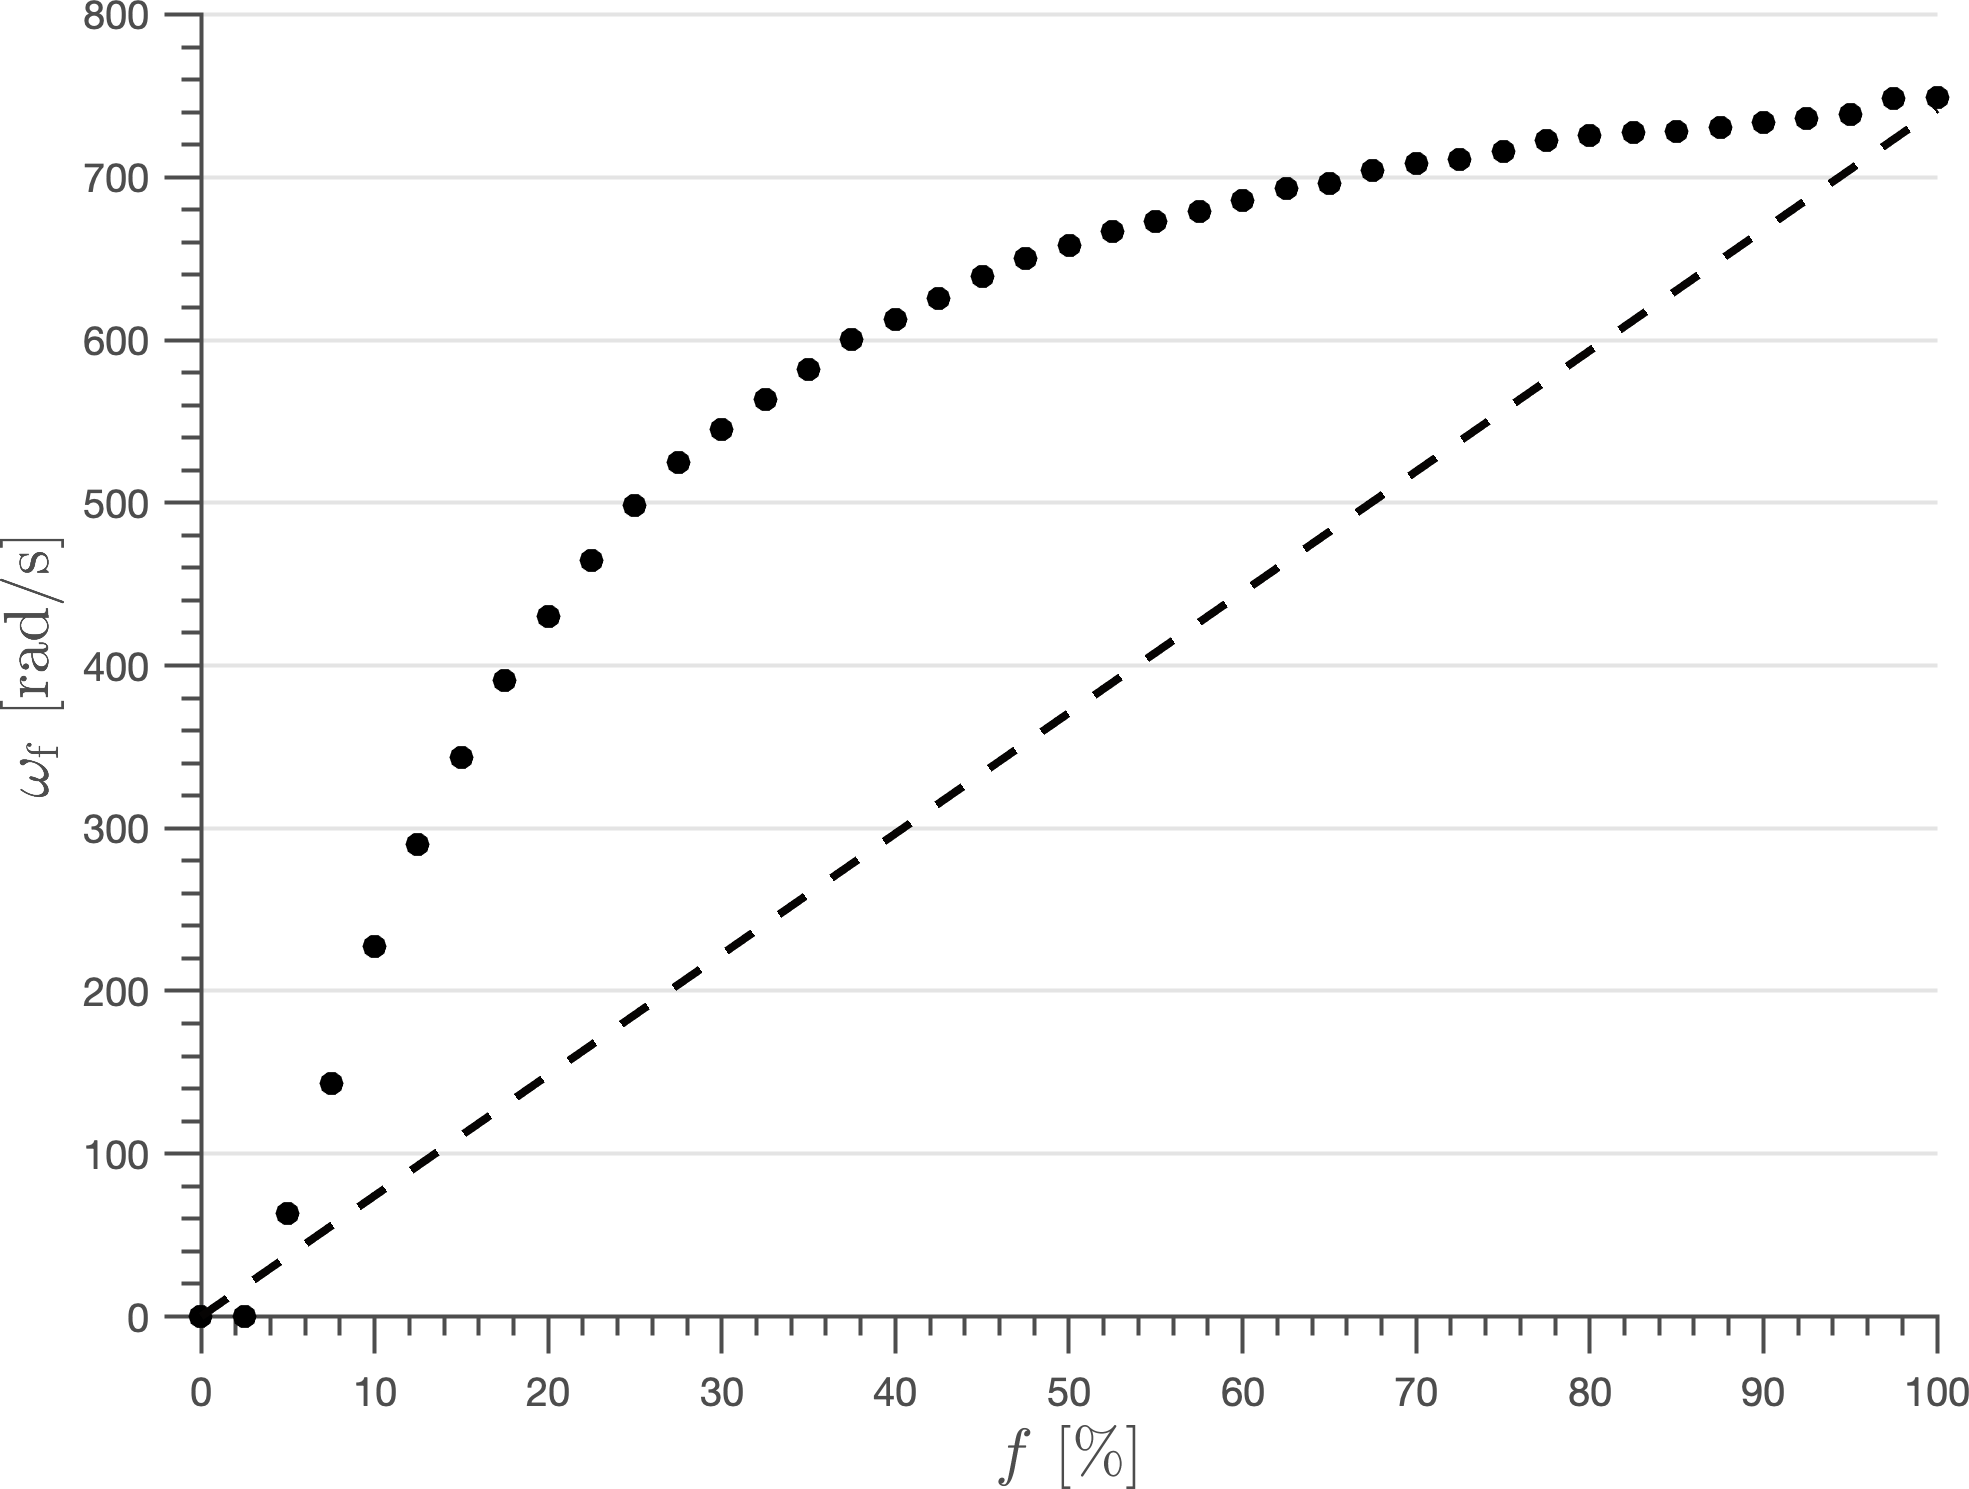
\includegraphics[width=14cm]{images/motor_pwm_response20.png}
    \caption{A motor állandósult sebessége és a kitöltési tényező viszonya 20 kHz-es PWM jellel.}\label{fig:motor_response_20khz}
    \end{center}
\end{figure}

Az \ref{fig:speed_profile}. ábrával ellentétben a maximális sebesség nagyobb volt, mivel a 
terhelésként használt propeller ekkor még nem került a motorra. A szabályozó tervezése során alapfeltevés volt, hogy 
a motorra kapcsolt feszültség változatlan marad, ha a szabályozó kimenete állandó. Láthatóan a motor máshogy viselkedik 
a PWM jel hatására, mintha a PWM jel átlagfeszültségével megegyező nagyságú állandó feszültség lenne a motorra kapcsolva.
Ennek a jelenségnek a magyarázatához elég a \ref{chap:physical_system}. fejezetben bevezetett lineáris modell válaszát 
megvizsgálni PWM bemenetre. A PWM jel két részre bontható. Az első szakasz változtatható szélességű és a 
kimeneti feszültség maximum, a második szakaszban a kimeneti feszültség zérus 
\begin{equation}
    V(t) = 
    \begin{cases}
        V_\RM{max} & \text{ha } kt_\RM p \le t < ft_\RM p + kt_\RM p \\
        0 & \text{ha } ft_\RM p + kt_\RM p \le t < (k+1)t_\RM p
    \end{cases}\,,
\end{equation}
ahol \(t_\RM p\) a jel periódusideje és \(f\) a kitöltési tényező.
A rotor áramának dinamikáját az \eqref{eq:armature_circuit} egyenlet írja le. 
Állandó feszültségre megoldva az idő és az áram szeparálásával
\begin{equation}
    \begin{split}
    \int_{t_0}^{t} dt &= \int_{i_0}^{i} \frac{L di}{V-K_\RM m\dot\theta - Ri}, \\
    t - t_0 &= -\frac{L}{R} \ln \frac{V-K_\RM m\dot\theta-Ri}{V-K_\RM m\dot\theta-Ri_0}, \\
    i(t) &= \frac{V-K_\RM m\dot\theta}{R}\left(1-e^{-\frac{t-t_0}{L/R}} \right) + i_0 e^{-\frac{t-t_0}{L/R}}. 
    \end{split}
\end{equation}
A megoldás során alkalmazott feltételezés, hogy a rotor forgási sebessége állandónak tekinthető állandósult esetben. 
Ez egy realisztikus feltételezés, hiszen a motor mechanikai időállandója nagyságrendekkel nagyobb a PWM jel periódusidejénél 
a vizsgált rendszerben. Ugyanebből a feltételezésből következik, hogy elég a motorra ható forgatónyomaték átlagát figyelembe venni, 
mely~\eqref{eq:lenz_torque} alapján arányos a tekercsárammal. Az átlag meghatározásához két esetet kell figyelembe venni. 
Az első esetben a tekercsáram nulláról indul és még kevesebb mint egy periódus alatt visszaesik nullára. Ez a továbbiakban szakaszos üzemmódnak 
lesz hívva. A másik eset, hogy a kiinduláskor nullától eltérő tekercsáram pontosan a periódus végén esik vissza a kiindulási értékére. 
Ez lesz a folytonos üzemmód. Az átlag meghatározásához fel lett használva az a feltételezés, hogy elegendő az előbb kapott 
exponenciális változást leíró formula lineáris közelítését felhasználni. A közelítés szerint 
\begin{equation}
    \begin{split}
        i(t) &= (i_\RM{max} - i_0)\frac{t}{ft_\RM p} + i_0, \\
        i_\RM{max} &= \frac{V-K_\RM m\dot\theta}{R}\left(1-e^{-\frac{ft_\RM p}{L/R}} \right) + i_0 e^{-\frac{ft_\RM p}{L/R}}
    \end{split}
\end{equation}
amíg a feszültség értéke maximum. Szakaszos üzemmódban meg kell határozni az áram nullára visszaeséséhez szükséges időt. 
Ez az előző egyenletek alapján 
\begin{equation}
    t_f = \frac{L}{R}\ln\left[\frac{V}{K_\RM m\dot\theta}\left(e^{-\frac{ft_\RM p}{L/R}} - 1\right) + 1\right]
\end{equation}
a periódus kezdetéhez viszonyítva.
A tekercsáram átlaga ez alapján belátható hogy a következő összefüggéssel közelíthető
\begin{equation}
    \begin{split}
    i_\RM{avg} &= \frac{1}{2}i_\RM{max}\frac{t_\RM f}{t_\RM p} \\
               &= \frac{1}{2}\frac{V-K_\RM m\dot\theta}{R}\left(1-e^{-\frac{ft_\RM p}{L/R}} \right)\frac{L}{t_\RM p R}\ln\left[\frac{V}{K_\RM m\dot\theta}\left(e^{-\frac{ft_\RM p}{L/R}} - 1\right) + 1\right].
    \end{split}
\end{equation}
Folytonos üzemmódban a kezdeti tekercsáramot kell meghatározni felhasználva, hogy \(t_\RM f = t_\RM p\).
Az előző formulák alapján 
\begin{equation}
    i_0 = \frac{V}{R}\frac{1-e^{\frac{ft_\RM p}{L/R}}}{1-e^{\frac{t_\RM p}{L/R}}} - \frac{K_\RM m\dot\theta}{R}.
\end{equation}
Ebben az esetben a tekercsáram átlaga pedig
\begin{equation}
    \begin{split}
    i_\RM{avg} &= \frac{1}{2}\left(i_\RM{max}-i_0\right) + i_0 \\
               &= \frac{1}{2}\left[\frac{V-K_\RM m\dot\theta}{R}\left(1-e^{-\frac{ft_\RM p}{L/R}} \right) + 
               \left(1+e^{-\frac{ft_\RM p}{L/R}} \right)
               \left(\frac{V}{R}\frac{1-e^{\frac{ft_\RM p}{L/R}}}{1-e^{\frac{t_\RM p}{L/R}}} - \frac{K_\RM m\dot\theta}{R}\right)\right].
    \end{split}
\end{equation}
A tekercsáram mindvégig pozitív marad, így kifejezhető a motor szögsebessége és a kitöltési tényező közötti 
kapcsolat folytonos üzemmódban 
\begin{equation}
    \dot\theta_\RM{crit} \le \frac{V}{K_\RM m}\frac{1-e^{\frac{ft_\RM p}{L/R}}}{1-e^{\frac{t_\RM p}{L/R}}}.
\end{equation}
Az átlag áramot behelyettesítve az \eqref{eq:rotor_dynamics} egyenletbe állandósult állapotban 
\begin{equation}
    B_\RM m\dot\theta = K_\RM m i_\RM{avg} + \tau_\RM e,
\end{equation}
ahol \(\tau_\RM e\) itt a statikus súrlódást fogja modellezni. Láthatóan létezik egy minimum kitöltési tényező 
ami alatt el sem indul a motor. 
Az \ref{fig:motor_response_20khz_with_model}. ábrán látható a 20kHz-en mért válasz és a modell által megjósolt viselkedés. 
A szaggatott görbe a kritikus szögsebességet jelöli, amely alatt folytonos üzemmódba lép át a rendszer. Felette pedig szakaszos üzemmódban működik. 

\begin{figure}[t!]
    \begin{center}
    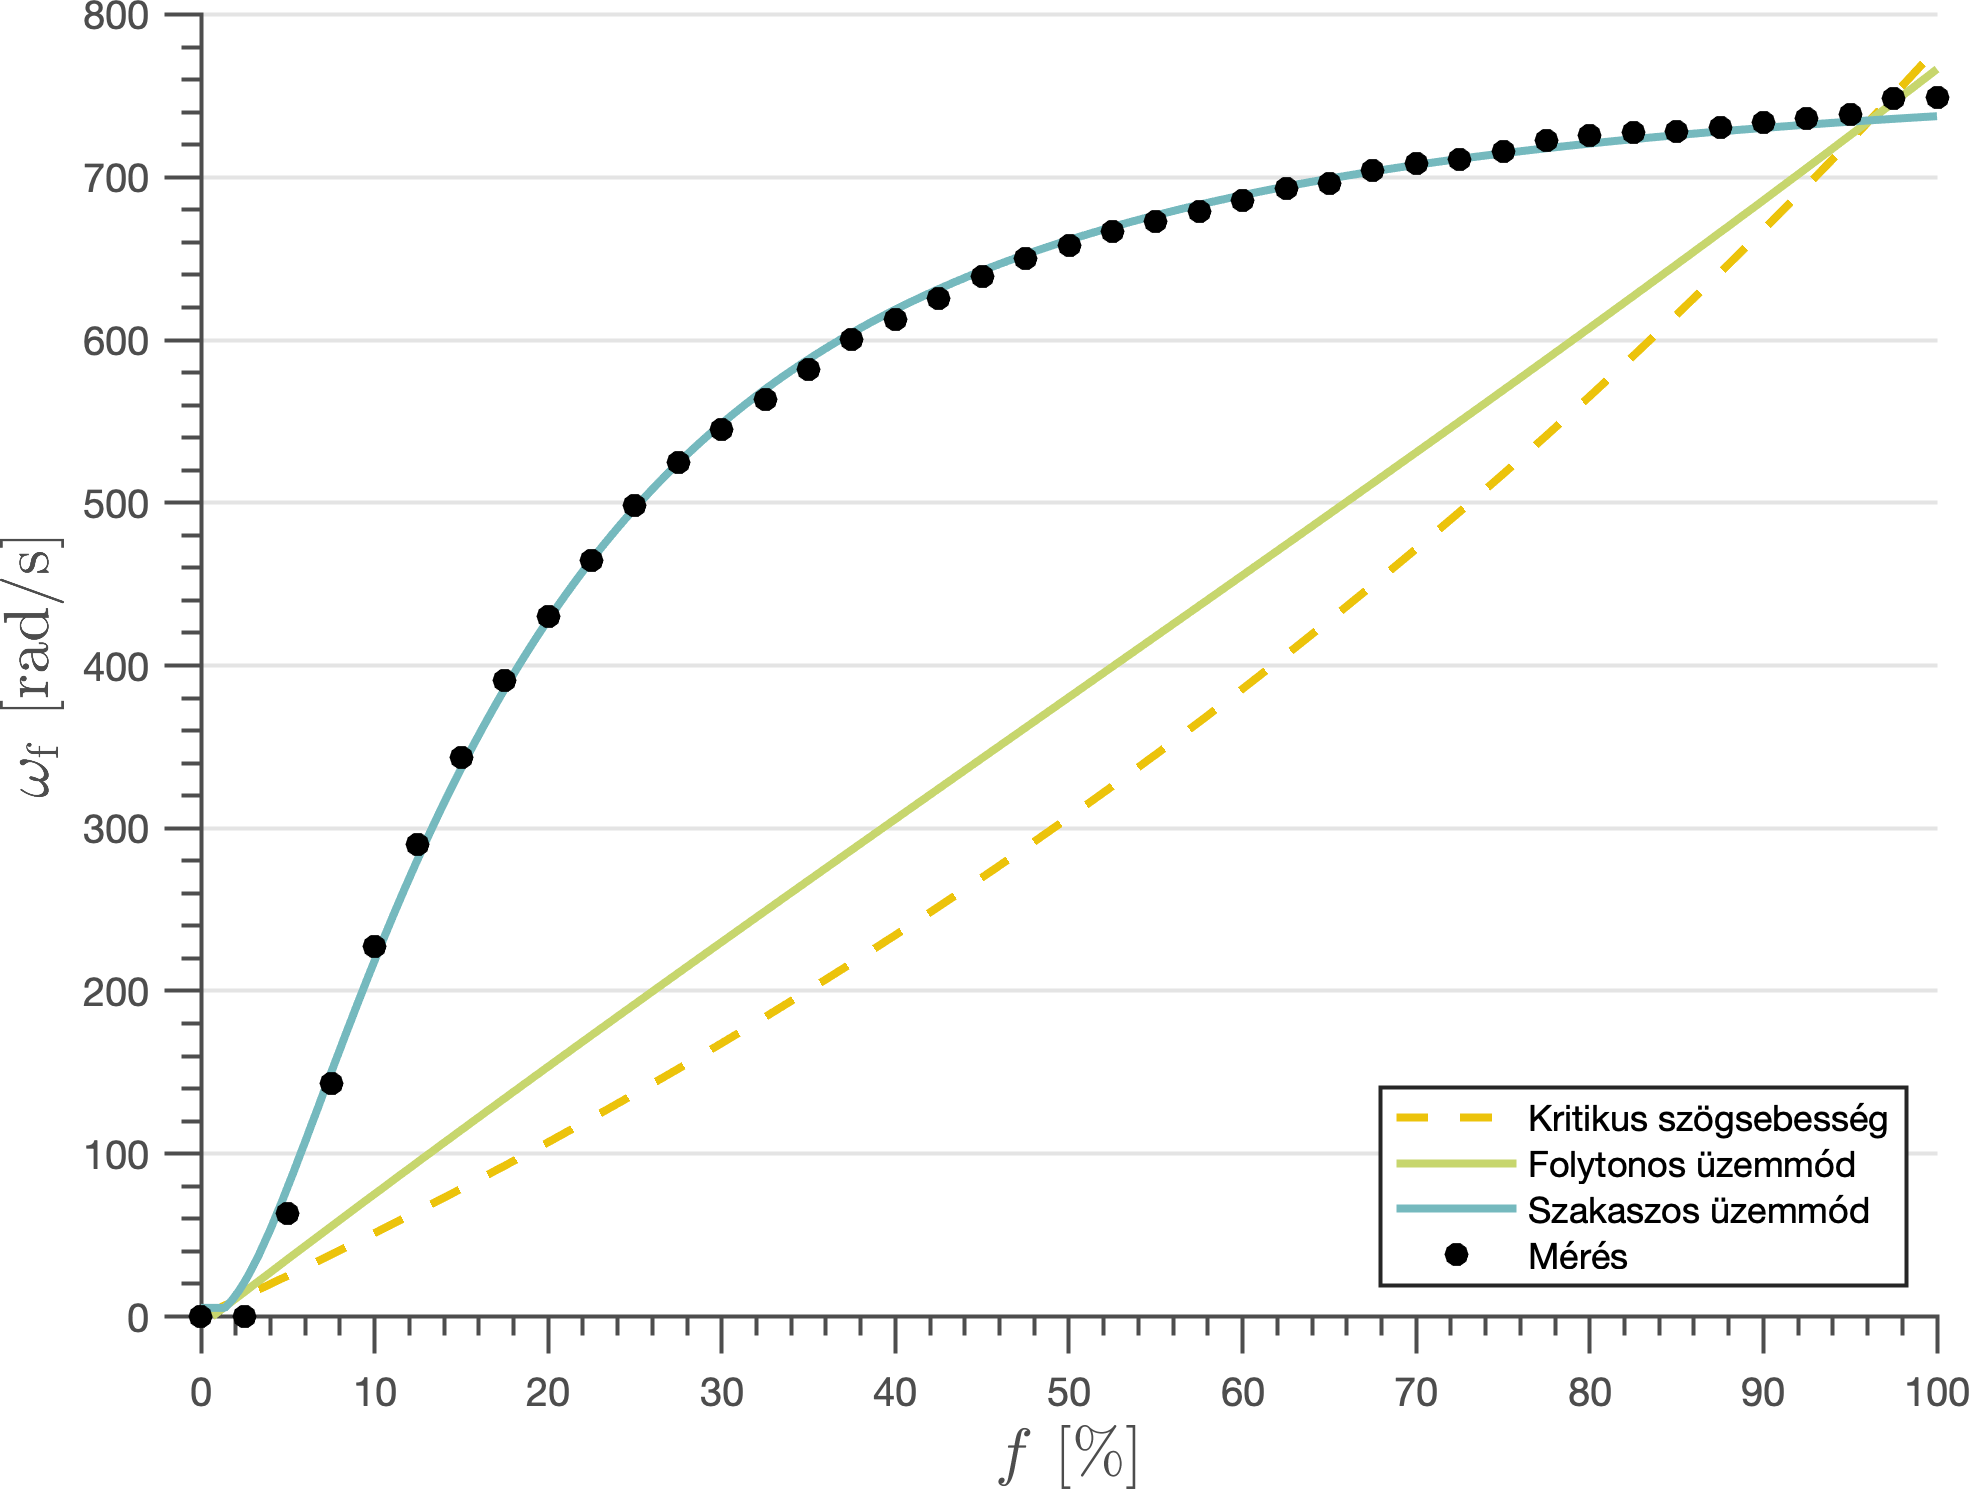
\includegraphics[width=\textwidth]{images/motor_pwm_response20_with_model.png}
    \caption{A motor állandósult sebessége és a kitöltési tényező viszonya modellekkel kiegészítve, 20 kHz-es PWM jellel.}\label{fig:motor_response_20khz_with_model}
    \end{center}
\end{figure}

A statikus súrlódásból származó nyomatékra \(\tau_\RM e = 1.5 \times 10^{-4}~\RM{Nm}\), a viszkózus csillapítási együtthatóra pedig 
\(B_\RM m = 2.7 \times 10^{-7}~\RM{kg \cdot m^2 \cdot s^{-1}}\) lett behelyettesítve. A többi paraméter az adatlapból származik. 
A mérés külső terhelés vagy hozzáadott tehetetlenség nélkül történt. Az egyezés jól látható, és az is látszik, hogy majdnem a 
teljes tartományon szakaszos üzemmódban működik a rendszer. A folytonos üzemmód viszont teljesen elfogadható 
lineáris viszonyt adna. A frekvencia és a viszkózus csillapítás növelésével el lehet érni, hogy a rendszer majdnem teljes 
egészében folytonos üzemmódban operáljon. A maxon ajánlása egyébként legalább 50 kHz használata a saját motorjaiknál, 
de ehhez nem adnak bővebb indoklást. Egy másik lehetőség a tekercs induktivitásának megnövelése például egy sorba kötött kis 
induktivitású folytótekerccsel. Ennek a módszernek viszont jóval kisebb hatása van a linearitásra a frekvenciához vagy a 
viszkeozus csillapítási együtthatóhoz képest. Még érdekesebb módszer lehet a súrlódás megnövelése. Ez ugyanúgy linearizálja a rendszert. 
Lehetnek alkalmazások, ahol ez az optimális megoldás. 

\chapter{Adatlapok}
\begin{figure}[H]
    \begin{center}
    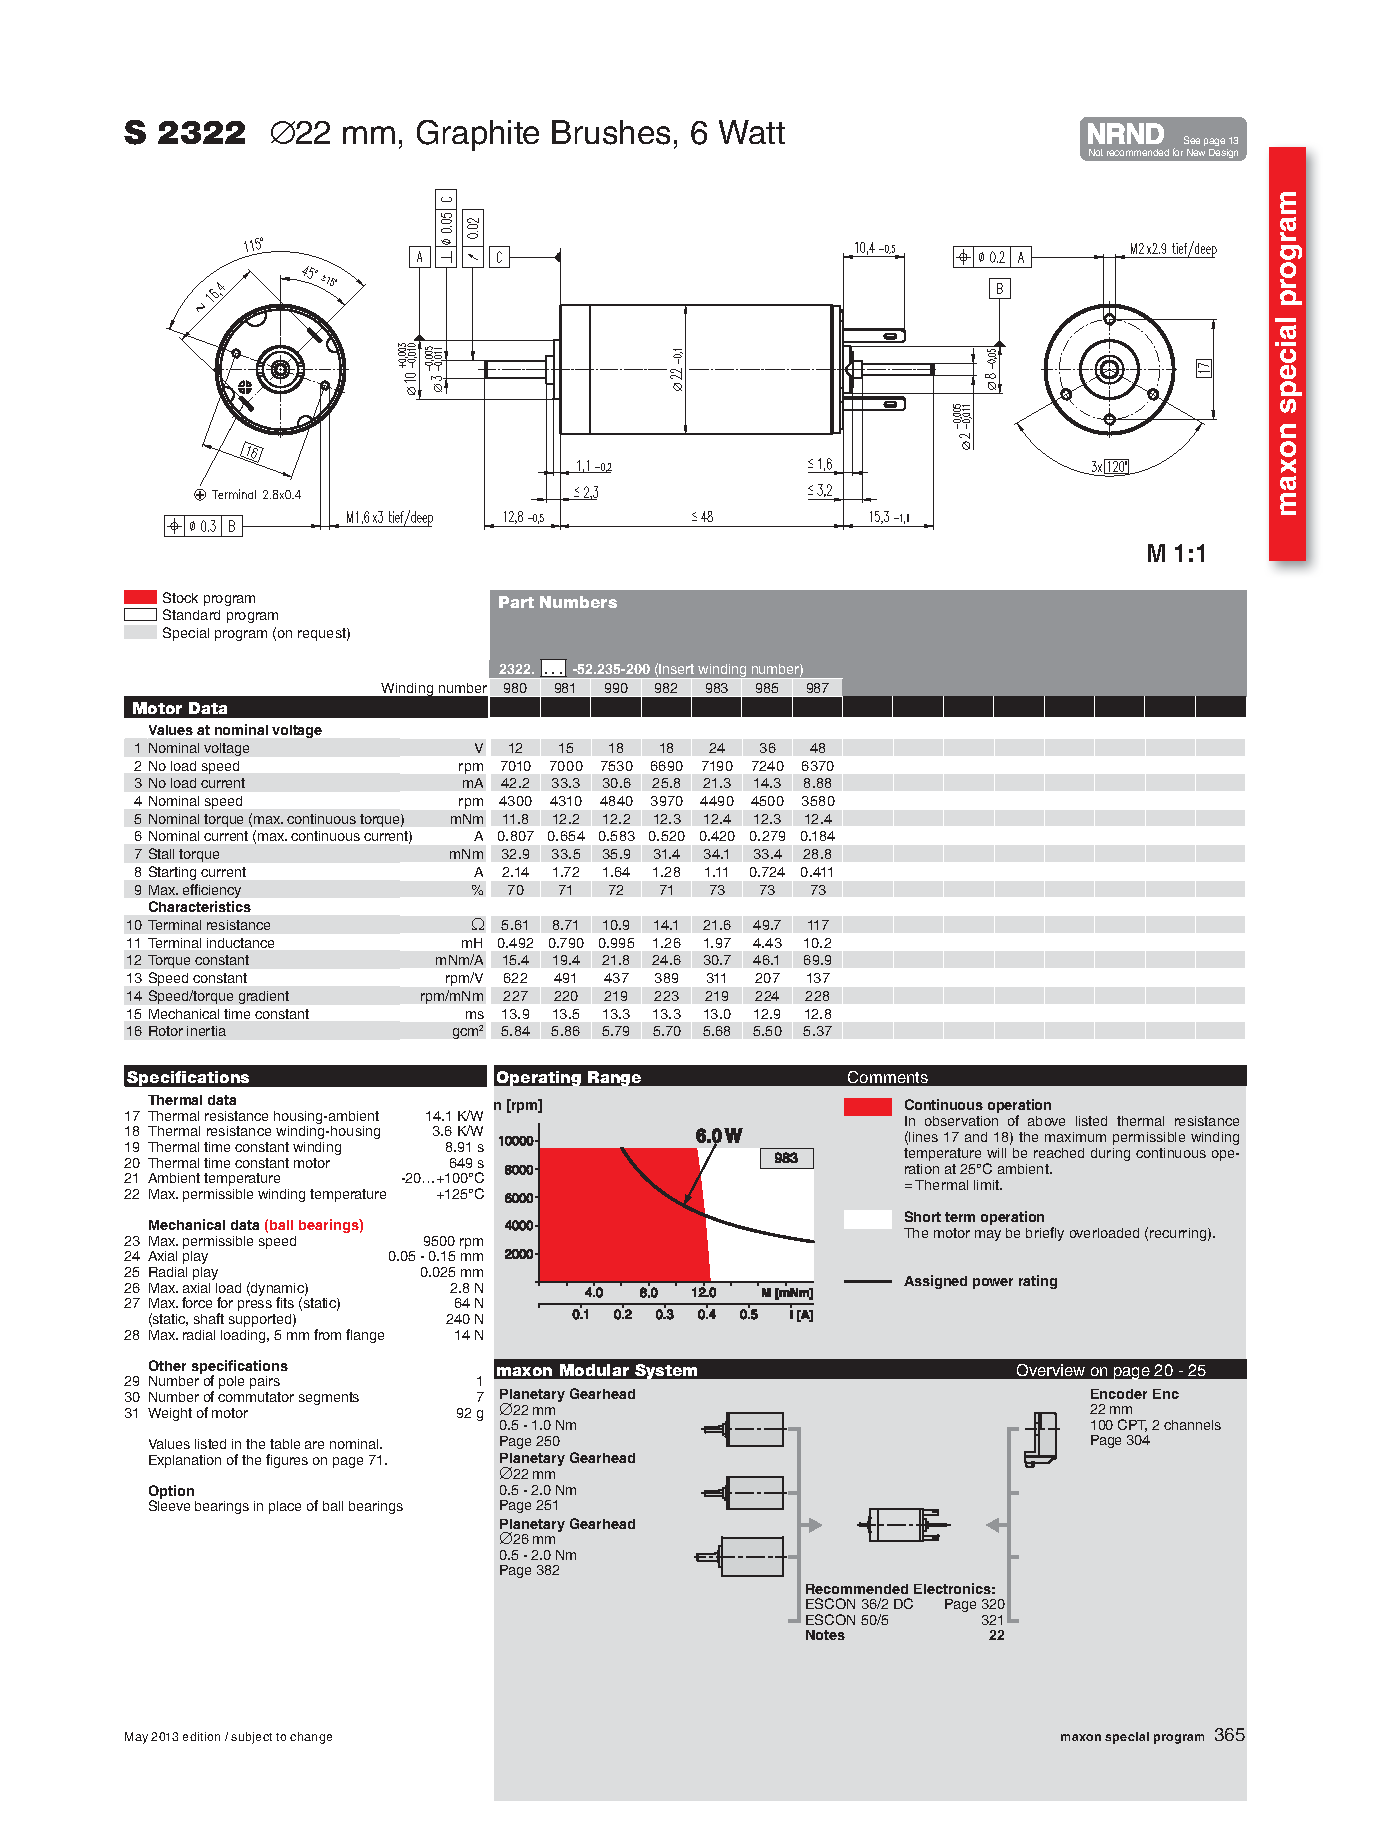
\includegraphics[width=\textwidth]{images/motor.pdf}
    \caption{Motor adatlap}\label{fig:motor_datasheet}
    \end{center}
\end{figure}

\begin{figure}[H]
    \begin{center}
    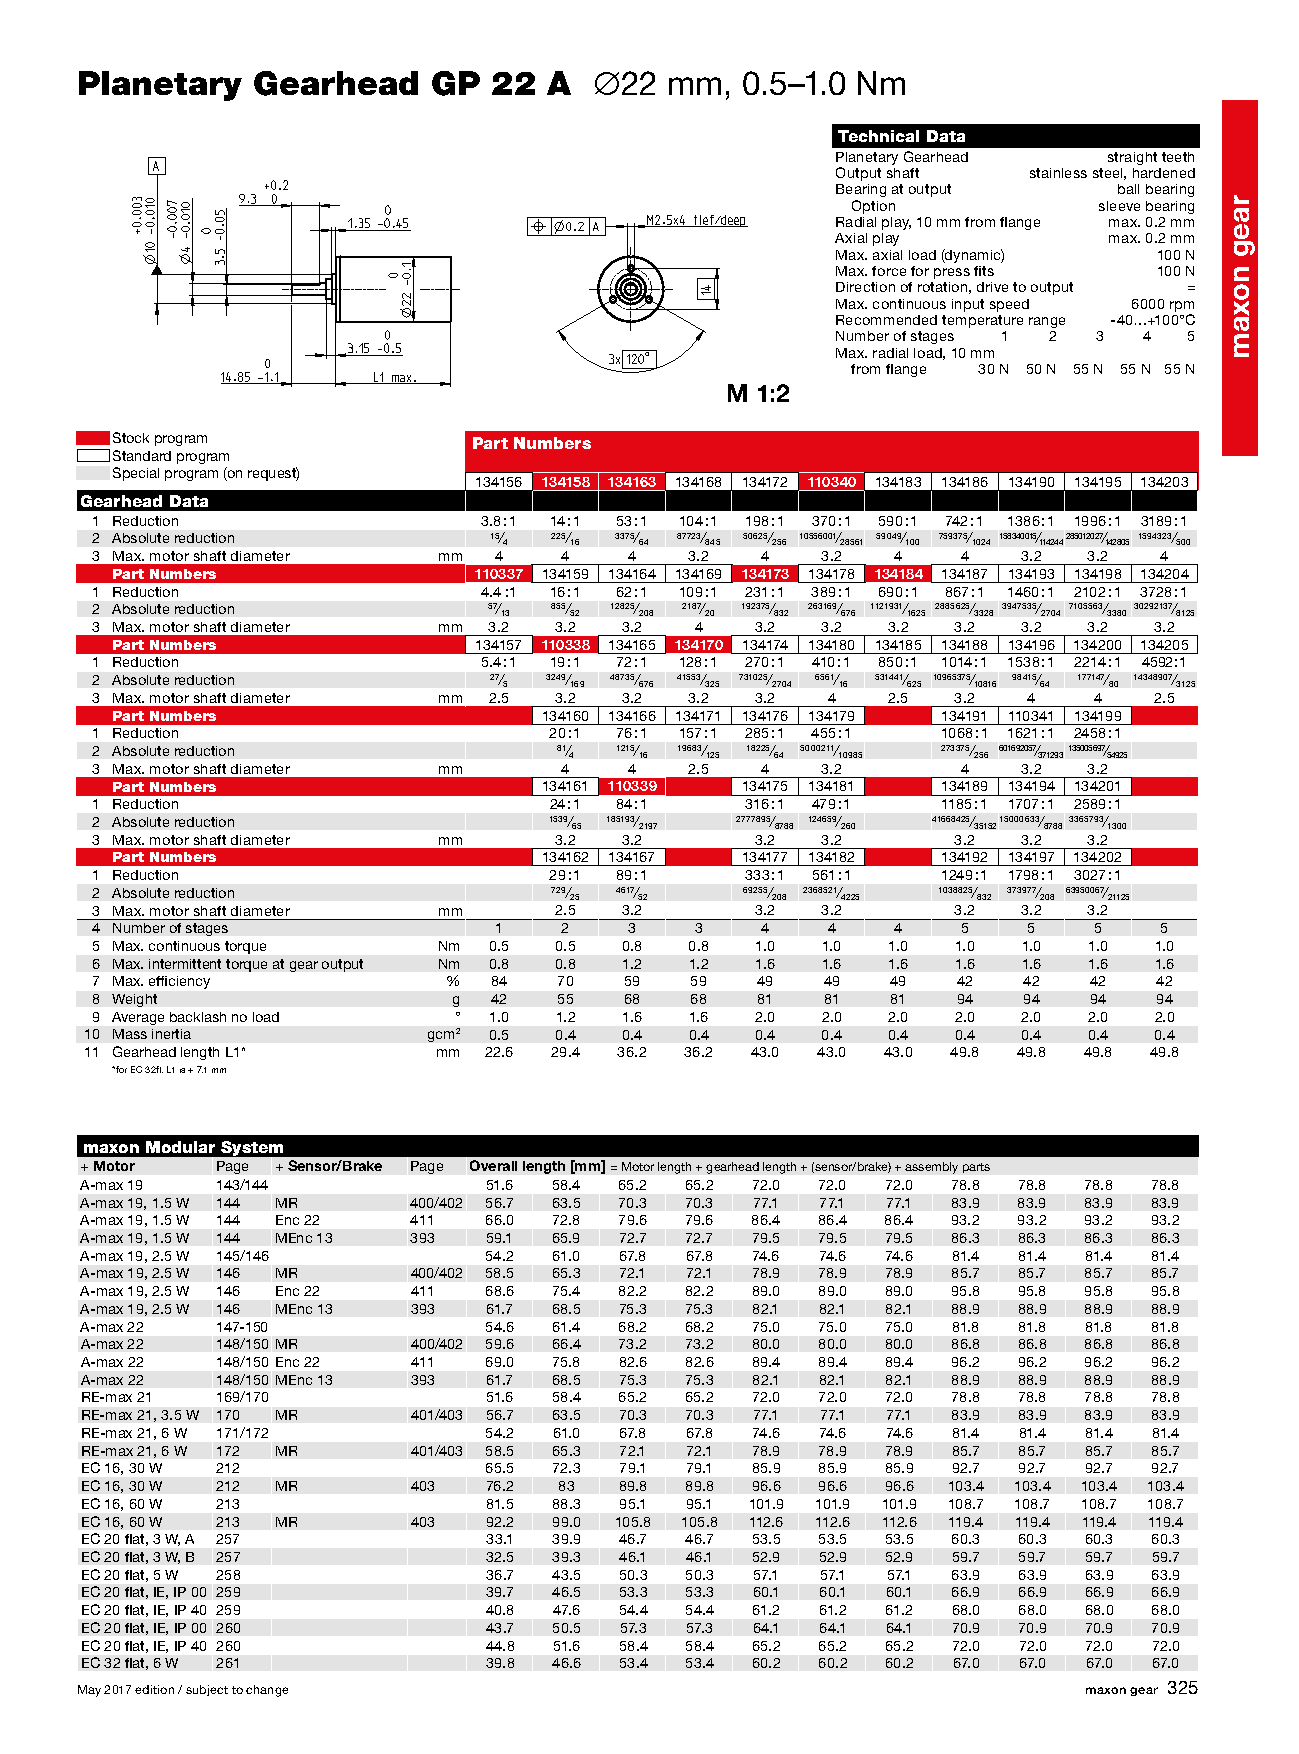
\includegraphics[width=\textwidth]{images/gearhead.pdf}
    \caption{Hajtómű adatlap}\label{fig:gearhead_datasheet}
    \end{center}
\end{figure}

\begin{figure}[H]
    \begin{center}
    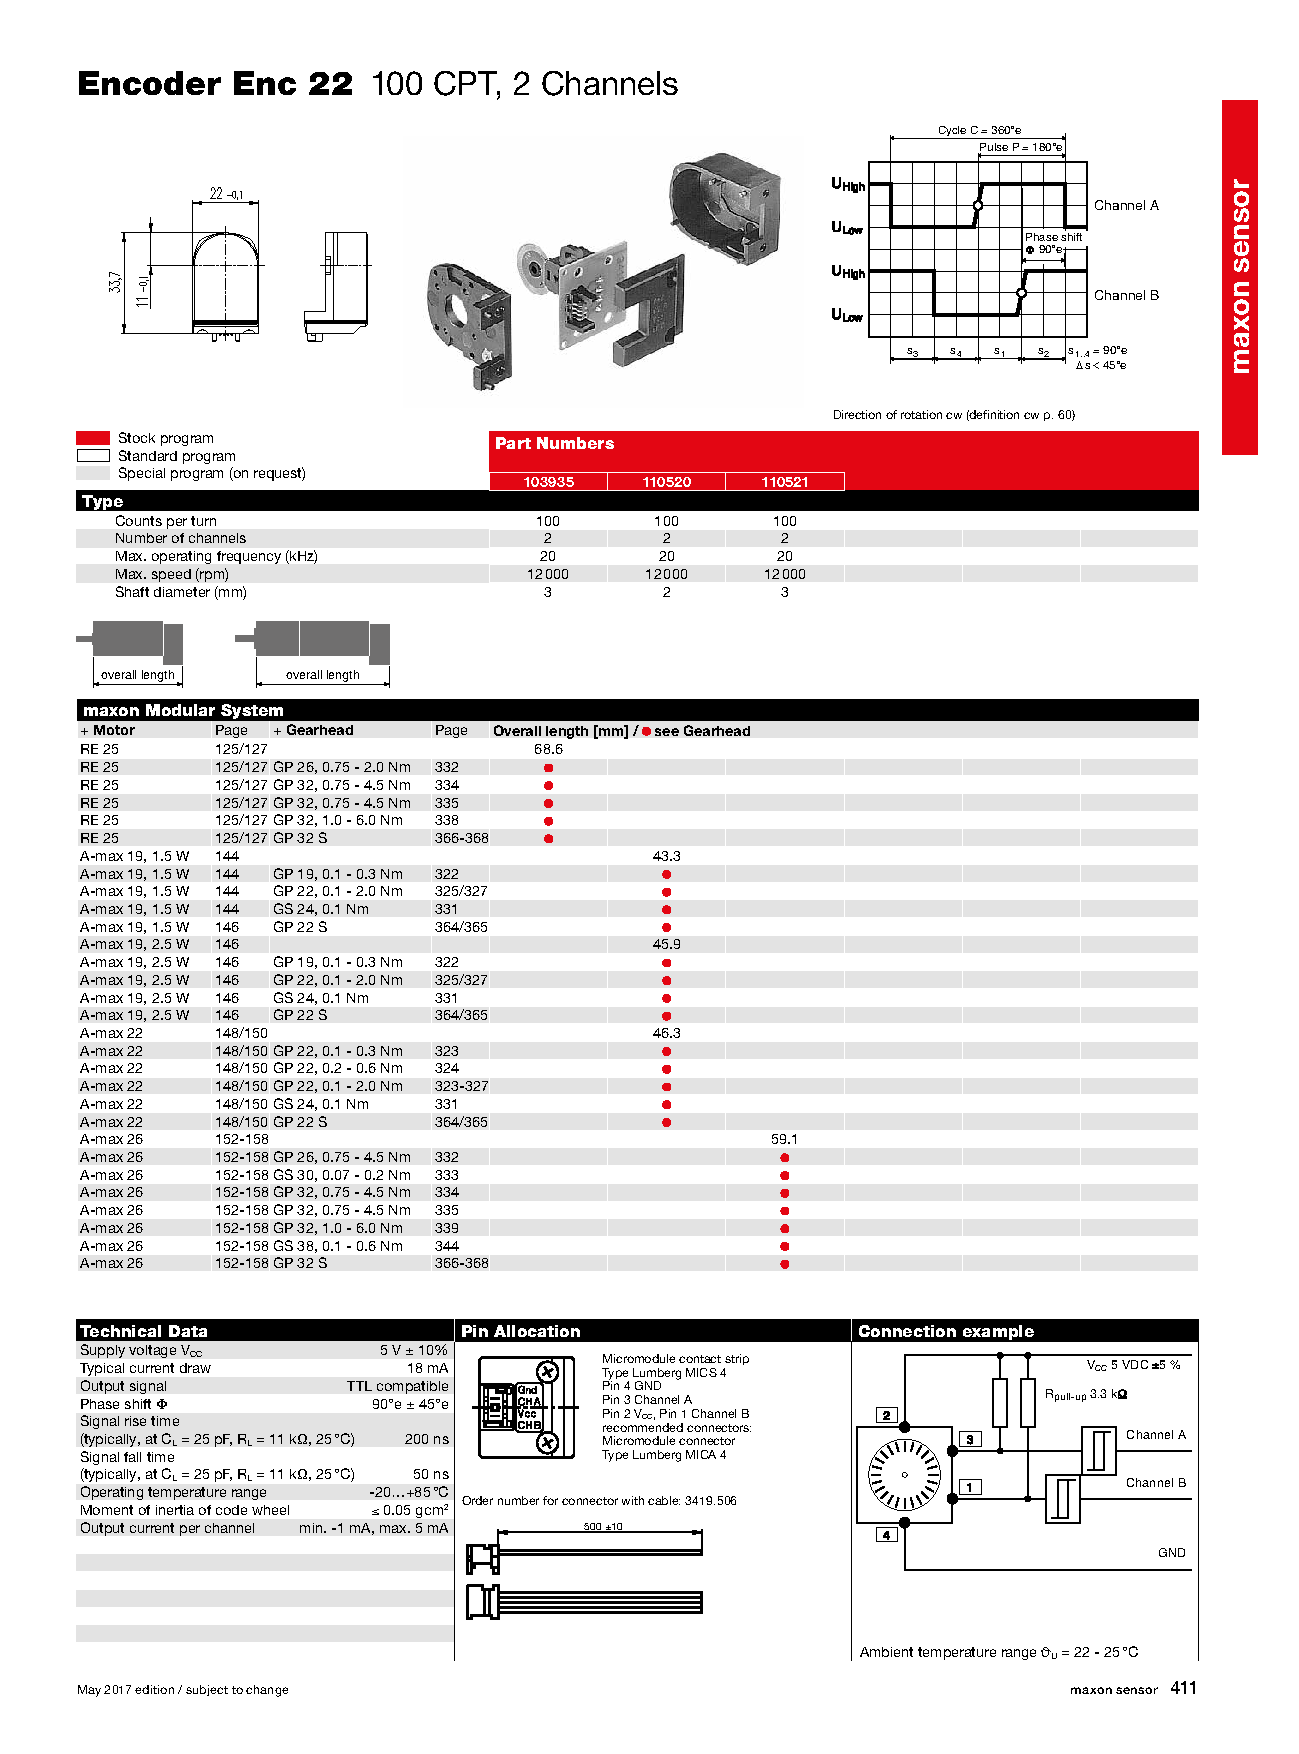
\includegraphics[width=\textwidth]{images/encoder.pdf}
    \caption{Enkóder adatlap}\label{fig:encoder_datasheet}
    \end{center}
\end{figure}

% \begin{table}[H]
%     \small\centering
%     \caption{Motor végsebesség és kapocsfeszültség mérések}\label{tab:speed_profile}
%     \tabcolsep=2pt
%     \begin{tabular}{d{-1}>{~}d{-1}>{~}d{-1}>{~}d{-1}}
%         \toprule
%         \multicolumn{1}{c}{Sajátkörfrekvencia [rad/s]} & \multicolumn{1}{c}{ []} & \multicolumn{1}{c}{ []} & \multicolumn{1}{c}{Hiba [ms]} \\ 
%         \multicolumn{1}{c}{\(\omega_\RM 0\)} & \multicolumn{1}{c}{\(b_\RM e\)} & \multicolumn{1}{c}{\(t_\RM s\)} & \multicolumn{1}{c}{\(\delta t_\RM s\)} \\
%         \midrule
%         6.12 & 6.12 & - & - \\
%         6.12 & 9.18 & - & - \\
%         6.12 & 12.24 & - & - \\
%         7.65 & 9.18 & - & - \\
%         7.65 & 12.24 & - & - \\
%         7.65 & 15.31 & - & - \\
%         7.65 & 18.37 & - & - \\
%         9.18 & 9.18 & - & - \\
%         9.18 & 12.24 & - & - \\
%         9.18 & 15.31 & 500 & 10 \\
%         9.18 & 18.37 & - & - \\
%         9.18 & 21.43 & - & - \\
%         9.18 & 24.49 & - & - \\
%         9.18 & 27.55 & - & - \\
%         10.71 & 9.18 & - & - \\
%         10.71 & 12.24 & - & - \\
%         10.71 & 15.31 & - & - \\
%         10.71 & 18.37 & - & - \\
%         10.71 & 21.43 & 415 & 4 \\
%         10.71 & 24.49 & - & - \\
%         10.71 & 27.55 & - & - \\
%         10.71 & 30.61 & - & - \\
%         10.71 & 33.67 & - & - \\
%         10.71 & 36.73 & - & - \\
%         12.24 & 9.18 & - & - \\
%         12.24 & 12.24 & 540 & 70 \\
%         12.24 & 15.31 & - & - \\
%         12.24 & 18.37 & 232 & 2 \\
%         12.24 & 21.43 & 460 & 40 \\
%         12.24 & 24.49 & - & - \\
%         12.24 & 27.55 & - & - \\
%         12.24 & 30.61 & 439 & 6 \\
%         12.24 & 33.67 & - & - \\
%         12.24 & 36.73 & - & - \\
%         12.24 & 39.80 & - & - \\
%         12.24 & 42.86 & - & - \\
%         12.24 & 45.92 & - & - \\
%         13.78 & 9.18 & - & - \\
%         13.78 & 12.24 & 363 & 2 \\
%         13.78 & 15.31 & 396 & 9 \\
%         13.78 & 18.37 & 280 & 20 \\
%         13.78 & 21.43 & 217.6 & 0.5 \\
%         13.78 & 24.49 & 257 & 1 \\
%         13.78 & 27.55 & 370 & 40 \\
%         13.78 & 30.61 & - & - \\
%         13.78 & 33.67 & - & - \\
%         13.78 & 36.73 & 370 & 10 \\
%         13.78 & 39.80 & - & - \\
%         13.78 & 42.86 & - & - \\
%         13.78 & 45.92 & - & - \\
%         13.78 & 48.98 & - & - \\
%         13.78 & 52.04 & - & - \\
%         13.78 & 55.10 & - & - \\
%         13.78 & 58.16 & - & - \\
%         15.31 & 9.18 & 545 & 3 \\
%         15.31 & 12.24 & - & - \\
%         15.31 & 15.31 & 325 & 3 \\
%         15.31 & 18.37 & 337 & 9 \\
%         15.31 & 21.43 & 170.8 & 0.5 \\
%         15.31 & 24.49 & 210 & 10 \\
%         15.31 & 27.55 & 230.1 & 0.8 \\
%         15.31 & 30.61 & 280 & 30 \\
%         15.31 & 33.67 & 430 & 30 \\
%         15.31 & 36.73 & - & - \\
%         15.31 & 39.80 & - & - \\
%         15.31 & 42.86 & 326 & 2 \\
%         15.31 & 45.92 & 372 & 7 \\
%         15.31 & 48.98 & - & - \\
%         15.31 & 52.04 & - & - \\
%         15.31 & 55.10 & - & - \\
%         15.31 & 58.16 & - & - \\
%         15.31 & 61.22 & - & - \\
%         15.31 & 64.29 & - & - \\
%         15.31 & 67.35 & - & - \\
%         16.84 & 9.18 & - & - \\
%         16.84 & 12.24 & - & - \\
%         16.84 & 15.31 & - & - \\
%         16.84 & 18.37 & 302 & 5 \\
%         16.84 & 21.43 & 255 & 5 \\
%         16.84 & 24.49 & 162 & 1 \\
%         16.84 & 27.55 & 184 & 1 \\
%         16.84 & 30.61 & 212 & 2 \\
%         16.84 & 33.67 & 231 & 2 \\
%         16.84 & 36.73 & 280 & 20 \\
%         16.84 & 39.80 & 390 & 40 \\
%         16.84 & 42.86 & - & - \\
%         16.84 & 45.92 & - & - \\
%         16.84 & 48.98 & - & - \\
%         16.84 & 52.04 & 317 & 6 \\
%         16.84 & 55.10 & 336 & 7 \\
%         16.84 & 58.16 & - & - \\
%         16.84 & 61.22 & - & - \\
%         16.84 & 64.29 & - & - \\
%         16.84 & 67.35 & - & - \\
%         16.84 & 70.41 & - & - \\
%         16.84 & 73.47 & - & - \\
%         16.84 & 76.53 & - & - \\
%         16.84 & 79.59 & - & - \\
%         18.37 & 9.18 & - & - \\
%         18.37 & 12.24 & - & - \\
%         18.37 & 15.31 & - & - \\
%         18.37 & 18.37 & 268 & 2 \\
%         18.37 & 21.43 & 271 & 4 \\
%         18.37 & 24.49 & 217 & 7 \\
%         18.37 & 27.55 & 142.4 & 0.7 \\
%         18.37 & 30.61 & 160 & 1 \\
%         18.37 & 33.67 & 174.8 & 0.4 \\
%         18.37 & 36.73 & 260 & 30 \\
%         18.37 & 39.80 & 300 & 40 \\
%         18.37 & 42.86 & 320 & 40 \\
%         18.37 & 45.92 & - & - \\
%         18.37 & 48.98 & - & - \\
%         18.37 & 52.04 & - & - \\
%         18.37 & 55.10 & - & - \\
%         18.37 & 58.16 & - & - \\
%         18.37 & 61.22 & - & - \\
%         18.37 & 64.29 & - & - \\
%         18.37 & 67.35 & - & - \\
%         18.37 & 70.41 & - & - \\
%         18.37 & 73.47 & - & - \\
%         18.37 & 76.53 & - & - \\
%         18.37 & 79.59 & - & - \\
%         18.37 & 82.65 & - & - \\
%         18.37 & 85.71 & - & - \\
%         18.37 & 88.78 & - & - \\
%         18.37 & 91.84 & - & - \\
%         19.90 & 9.18 & 555 & 3 \\
%         19.90 & 12.24 & 430 & 20 \\
%         19.90 & 15.31 & - & - \\
%         19.90 & 18.37 & - & - \\
%         19.90 & 21.43 & 248 & 2 \\
%         19.90 & 24.49 & - & - \\
%         19.90 & 27.55 & - & - \\
%         19.90 & 30.61 & 137.7 & 0.8 \\
%         19.90 & 33.67 & 151 & 1 \\
%         19.90 & 36.73 & 174 & 2 \\
%         19.90 & 39.80 & 210 & 10 \\
%         19.90 & 42.86 & 210 & 2 \\
%         19.90 & 45.92 & 250 & 20 \\
%         19.90 & 48.98 & 320 & 40 \\
%         19.90 & 52.04 & 310 & 30 \\
%         19.90 & 55.10 & - & - \\
%         19.90 & 58.16 & - & - \\
%         19.90 & 61.22 & - & - \\
%         19.90 & 64.29 & - & - \\
%         19.90 & 67.35 & 330 & 30 \\
%         19.90 & 70.41 & 280 & 6 \\
%         19.90 & 73.47 & 283 & 5 \\
%         19.90 & 76.53 & - & - \\
%         19.90 & 79.59 & - & - \\
%         19.90 & 82.65 & - & - \\
%         19.90 & 85.71 & - & - \\
%         19.90 & 88.78 & - & - \\
%         19.90 & 91.84 & - & - \\
%         19.90 & 94.90 & - & - \\
%         19.90 & 97.96 & - & - \\
%         19.90 & 101.02 & - & - \\
%         19.90 & 104.08 & - & - \\
%         21.43 & 12.24 & - & - \\
%         21.43 & 15.31 & - & - \\
%         21.43 & 18.37 & - & - \\
%         21.43 & 21.43 & - & - \\
%         21.43 & 24.49 & 237 & 4 \\
%         21.43 & 27.55 & 231 & 8 \\
%         21.43 & 30.61 & 140 & 10 \\
%         21.43 & 33.67 & 128 & 1 \\
%         21.43 & 36.73 & 140 & 1 \\
%         21.43 & 39.80 & 170 & 10 \\
%         21.43 & 42.86 & 180 & 2 \\
%         21.43 & 45.92 & 189 & 1 \\
%         21.43 & 48.98 & 210 & 20 \\
%         21.43 & 52.04 & 270 & 30 \\
%         21.43 & 55.10 & 320 & 40 \\
%         21.43 & 58.16 & 310 & 30 \\
%         21.43 & 61.22 & 360 & 30 \\
%         21.43 & 64.29 & - & - \\
%         21.43 & 67.35 & - & - \\
%         21.43 & 70.41 & - & - \\
%         21.43 & 73.47 & - & - \\
%         21.43 & 76.53 & - & - \\
%         21.43 & 79.59 & 253 & 5 \\
%         21.43 & 82.65 & 280 & 10 \\
%         21.43 & 85.71 & 277 & 8 \\
%         21.43 & 88.78 & - & - \\
%         21.43 & 91.84 & - & - \\
%         21.43 & 94.90 & - & - \\
%         21.43 & 97.96 & - & - \\
%         21.43 & 101.02 & - & - \\
%         21.43 & 104.08 & - & - \\
%         21.43 & 107.14 & - & - \\
%         21.43 & 110.20 & - & - \\
%         21.43 & 113.27 & - & - \\
%         21.43 & 116.33 & - & - \\
%         21.43 & 119.39 & - & - \\
%         22.96 & 12.24 & - & - \\
%         22.96 & 15.31 & - & - \\
%         22.96 & 18.37 & - & - \\
%         22.96 & 21.43 & - & - \\
%         22.96 & 24.49 & - & - \\
%         22.96 & 27.55 & - & - \\
%         22.96 & 30.61 & - & - \\
%         22.96 & 33.67 & 170 & 20 \\
%         22.96 & 36.73 & 119.2 & 0.6 \\
%         22.96 & 39.80 & 131 & 1 \\
%         22.96 & 42.86 & 140 & 1 \\
%         22.96 & 45.92 & 157 & 2 \\
%         22.96 & 48.98 & 170 & 2 \\
%         22.96 & 52.04 & 180 & 2 \\
%         22.96 & 55.10 & - & - \\
%         22.96 & 58.16 & - & - \\
%         22.96 & 61.22 & 320 & 30 \\
%         22.96 & 64.29 & 340 & 30 \\
%         22.96 & 67.35 & 300 & 40 \\
%         22.96 & 70.41 & - & - \\
%         22.96 & 73.47 & - & - \\
%         22.96 & 76.53 & - & - \\
%         22.96 & 79.59 & - & - \\
%         22.96 & 82.65 & - & - \\
%         22.96 & 85.71 & - & - \\
%         22.96 & 88.78 & 340 & 50 \\
%         22.96 & 91.84 & - & - \\
%         22.96 & 94.90 & - & - \\
%         22.96 & 97.96 & - & - \\
%         22.96 & 101.02 & - & - \\
%         22.96 & 104.08 & - & - \\
%         22.96 & 107.14 & - & - \\
%         22.96 & 110.20 & - & - \\
%         22.96 & 113.27 & - & - \\
%         22.96 & 116.33 & - & - \\
%         22.96 & 119.39 & - & - \\
%         22.96 & 122.45 & - & - \\
%         22.96 & 125.51 & - & - \\
%         22.96 & 128.57 & - & - \\
%         22.96 & 131.63 & - & - \\
%         24.49 & 15.31 & - & - \\
%         24.49 & 18.37 & - & - \\
%         24.49 & 21.43 & - & - \\
%         24.49 & 24.49 & - & - \\
%         24.49 & 27.55 & - & - \\
%         24.49 & 30.61 & - & - \\
%         24.49 & 33.67 & - & - \\
%         24.49 & 36.73 & - & - \\
%         24.49 & 39.80 & - & - \\
%         24.49 & 42.86 & - & - \\
%         24.49 & 45.92 & - & - \\
%         24.49 & 48.98 & - & - \\
%         24.49 & 52.04 & - & - \\
%         24.49 & 55.10 & - & - \\
%         24.49 & 58.16 & - & - \\
%         24.49 & 61.22 & - & - \\
%         24.49 & 64.29 & - & - \\
%         24.49 & 67.35 & - & - \\
%         24.49 & 70.41 & - & - \\
%         24.49 & 73.47 & - & - \\
%         24.49 & 76.53 & - & - \\
%         24.49 & 79.59 & - & - \\
%         24.49 & 82.65 & - & - \\
%         24.49 & 85.71 & - & - \\
%         24.49 & 88.78 & - & - \\
%         24.49 & 91.84 & - & - \\
%         24.49 & 94.90 & - & - \\
%         24.49 & 97.96 & - & - \\
%         24.49 & 101.02 & - & - \\
%         24.49 & 104.08 & - & - \\
%         24.49 & 107.14 & - & - \\
%         24.49 & 110.20 & - & - \\
%         24.49 & 113.27 & - & - \\
%         24.49 & 116.33 & 241 & 6 \\
%         24.49 & 119.39 & 270 & 10 \\
%         24.49 & 122.45 & 290 & 20 \\
%         24.49 & 125.51 & 248 & 4 \\
%         24.49 & 128.57 & - & - \\
%         24.49 & 131.63 & - & - \\
%         24.49 & 134.69 & - & - \\
%         24.49 & 137.76 & - & - \\
%         24.49 & 140.82 & - & - \\
%         24.49 & 143.88 & - & - \\
%         26.02 & 15.31 & 425 & 3 \\
%         26.02 & 18.37 & 410 & 30 \\
%         26.02 & 21.43 & - & - \\
%         26.02 & 24.49 & - & - \\
%         26.02 & 27.55 & - & - \\
%         26.02 & 30.61 & 210 & 20 \\
%         26.02 & 33.67 & 183 & 3 \\
%         26.02 & 36.73 & 173 & 7 \\
%         26.02 & 39.80 & 155 & 8 \\
%         26.02 & 42.86 & 107 & 7 \\
%         26.02 & 45.92 & 108.2 & 0.8 \\
%         26.02 & 48.98 & 116 & 1 \\
%         26.02 & 52.04 & 132 & 2 \\
%         26.02 & 55.10 & 143 & 3 \\
%         26.02 & 58.16 & 145 & 2 \\
%         26.02 & 61.22 & 154 & 1 \\
%         26.02 & 64.29 & 190 & 20 \\
%         26.02 & 67.35 & 200 & 20 \\
%         26.02 & 70.41 & - & - \\
%         26.02 & 73.47 & 280 & 30 \\
%         26.02 & 76.53 & 310 & 30 \\
%         26.02 & 79.59 & - & - \\
%         26.02 & 82.65 & - & - \\
%         26.02 & 85.71 & - & - \\
%         26.02 & 88.78 & - & - \\
%         26.02 & 91.84 & - & - \\
%         26.02 & 94.90 & - & - \\
%         26.02 & 97.96 & - & - \\
%         26.02 & 101.02 & - & - \\
%         26.02 & 104.08 & - & - \\
%         26.02 & 107.14 & - & - \\
%         26.02 & 110.20 & - & - \\
%         26.02 & 113.27 & - & - \\
%         26.02 & 116.33 & - & - \\
%         26.02 & 119.39 & 280 & 30 \\
%         26.02 & 122.45 & 270 & 30 \\
%         26.02 & 125.51 & 280 & 30 \\
%         26.02 & 128.57 & 240 & 20 \\
%         26.02 & 131.63 & 219 & 5 \\
%         26.02 & 134.69 & - & - \\
%         26.02 & 137.76 & - & - \\
%         26.02 & 140.82 & - & - \\
%         26.02 & 143.88 & - & - \\
%         26.02 & 146.94 & - & - \\
%         26.02 & 150.00 & - & - \\
%         27.55 & 18.37 & - & - \\
%         27.55 & 21.43 & - & - \\
%         27.55 & 24.49 & - & - \\
%         27.55 & 27.55 & - & - \\
%         27.55 & 30.61 & - & - \\
%         27.55 & 33.67 & - & - \\
%         27.55 & 36.73 & - & - \\
%         27.55 & 39.80 & - & - \\
%         27.55 & 42.86 & - & - \\
%         27.55 & 45.92 & - & - \\
%         27.55 & 48.98 & - & - \\
%         27.55 & 52.04 & - & - \\
%         27.55 & 55.10 & - & - \\
%         27.55 & 58.16 & - & - \\
%         27.55 & 61.22 & - & - \\
%         27.55 & 64.29 & - & - \\
%         27.55 & 67.35 & - & - \\
%         27.55 & 70.41 & - & - \\
%         27.55 & 73.47 & - & - \\
%         27.55 & 76.53 & - & - \\
%         27.55 & 79.59 & - & - \\
%         27.55 & 82.65 & - & - \\
%         27.55 & 85.71 & - & - \\
%         27.55 & 88.78 & - & - \\
%         27.55 & 91.84 & - & - \\
%         27.55 & 94.90 & - & - \\
%         27.55 & 97.96 & - & - \\
%         27.55 & 101.02 & - & - \\
%         27.55 & 104.08 & - & - \\
%         27.55 & 107.14 & - & - \\
%         27.55 & 110.20 & - & - \\
%         27.55 & 113.27 & - & - \\
%         27.55 & 116.33 & - & - \\
%         27.55 & 119.39 & - & - \\
%         27.55 & 122.45 & - & - \\
%         27.55 & 125.51 & - & - \\
%         27.55 & 128.57 & - & - \\
%         27.55 & 131.63 & - & - \\
%         27.55 & 134.69 & 270 & 30 \\
%         27.55 & 137.76 & - & - \\
%         27.55 & 140.82 & 270 & 30 \\
%         27.55 & 143.88 & 240 & 30 \\
%         27.55 & 146.94 & - & - \\
%         27.55 & 150.00 & 240 & 10 \\
%         29.08 & 18.37 & 400 & 2 \\
%         29.08 & 21.43 & 380 & 20 \\
%         29.08 & 24.49 & - & - \\
%         29.08 & 27.55 & - & - \\
%         29.08 & 30.61 & - & - \\
%         29.08 & 33.67 & - & - \\
%         29.08 & 36.73 & - & - \\
%         29.08 & 39.80 & - & - \\
%         29.08 & 42.86 & 169 & 5 \\
%         29.08 & 45.92 & 151 & 5 \\
%         29.08 & 48.98 & 125 & 9 \\
%         29.08 & 52.04 & 98 & 1 \\
%         29.08 & 55.10 & 106 & 1 \\
%         29.08 & 58.16 & 113 & 2 \\
%         29.08 & 61.22 & 118 & 2 \\
%         29.08 & 64.29 & 129 & 1 \\
%         29.08 & 67.35 & 139 & 2 \\
%         29.08 & 70.41 & 150 & 10 \\
%         29.08 & 73.47 & 210 & 30 \\
%         29.08 & 76.53 & - & - \\
%         29.08 & 79.59 & - & - \\
%         29.08 & 82.65 & 270 & 30 \\
%         29.08 & 85.71 & - & - \\
%         29.08 & 88.78 & - & - \\
%         29.08 & 91.84 & - & - \\
%         29.08 & 94.90 & - & - \\
%         29.08 & 97.96 & - & - \\
%         29.08 & 101.02 & - & - \\
%         29.08 & 104.08 & - & - \\
%         29.08 & 107.14 & - & - \\
%         29.08 & 110.20 & - & - \\
%         29.08 & 113.27 & - & - \\
%         29.08 & 116.33 & - & - \\
%         29.08 & 119.39 & - & - \\
%         29.08 & 122.45 & - & - \\
%         29.08 & 125.51 & - & - \\
%         29.08 & 128.57 & - & - \\
%         29.08 & 131.63 & - & - \\
%         29.08 & 134.69 & - & - \\
%         29.08 & 137.76 & - & - \\
%         29.08 & 140.82 & - & - \\
%         29.08 & 143.88 & - & - \\
%         29.08 & 146.94 & 240 & 30 \\
%         29.08 & 150.00 & - & - \\
%         30.61 & 24.49 & - & - \\
%         30.61 & 27.55 & - & - \\
%         30.61 & 30.61 & - & - \\
%         30.61 & 33.67 & - & - \\
%         30.61 & 36.73 & - & - \\
%         30.61 & 39.80 & - & - \\
%         30.61 & 42.86 & - & - \\
%         30.61 & 45.92 & - & - \\
%         30.61 & 48.98 & - & - \\
%         30.61 & 52.04 & - & - \\
%         30.61 & 55.10 & - & - \\
%         30.61 & 58.16 & - & - \\
%         30.61 & 61.22 & - & - \\
%         30.61 & 64.29 & - & - \\
%         30.61 & 67.35 & - & - \\
%         30.61 & 70.41 & - & - \\
%         30.61 & 73.47 & - & - \\
%         30.61 & 76.53 & 190 & 30 \\
%         30.61 & 79.59 & 230 & 20 \\
%         30.61 & 82.65 & 260 & 20 \\
%         30.61 & 85.71 & 260 & 20 \\
%         30.61 & 88.78 & 260 & 30 \\
%         30.61 & 91.84 & 240 & 30 \\
%         30.61 & 94.90 & 240 & 30 \\
%         30.61 & 97.96 & 270 & 30 \\
%         30.61 & 101.02 & 270 & 30 \\
%         30.61 & 104.08 & - & - \\
%         30.61 & 107.14 & - & - \\
%         30.61 & 110.20 & - & - \\
%         30.61 & 113.27 & - & - \\
%         30.61 & 116.33 & - & - \\
%         30.61 & 119.39 & - & - \\
%         30.61 & 122.45 & - & - \\
%         30.61 & 125.51 & - & - \\
%         30.61 & 128.57 & - & - \\
%         30.61 & 131.63 & - & - \\
%         30.61 & 134.69 & - & - \\
%         30.61 & 137.76 & - & - \\
%         30.61 & 140.82 & - & - \\
%         30.61 & 143.88 & - & - \\
%         30.61 & 146.94 & - & - \\
%         32.14 & 21.43 & 347 & 4 \\
%         32.14 & 24.49 & 340 & 30 \\
%         32.14 & 27.55 & - & - \\
%         32.14 & 30.61 & - & - \\
%         32.14 & 33.67 & - & - \\
%         32.14 & 36.73 & - & - \\
%         32.14 & 39.80 & - & - \\
%         32.14 & 42.86 & 149 & 2 \\
%         32.14 & 45.92 & 143 & 3 \\
%         32.14 & 48.98 & 127 & 3 \\
%         32.14 & 52.04 & 109 & 8 \\
%         32.14 & 55.10 & 104 & 9 \\
%         32.14 & 58.16 & 85.1 & 0.6 \\
%         32.14 & 61.22 & 100 & 10 \\
%         32.14 & 64.29 & 91.5 & 0.7 \\
%         32.14 & 67.35 & 95 & 1 \\
%         32.14 & 70.41 & 105 & 2 \\
%         32.14 & 73.47 & 110 & 2 \\
%         32.14 & 76.53 & 119 & 2 \\
%         32.14 & 79.59 & 119 & 2 \\
%         32.14 & 82.65 & 122 & 1 \\
%         32.14 & 85.71 & 150 & 20 \\
%         32.14 & 88.78 & 130 & 2 \\
%         32.14 & 91.84 & 190 & 30 \\
%         32.14 & 94.90 & 250 & 30 \\
%         32.14 & 97.96 & 220 & 20 \\
%         32.14 & 101.02 & 290 & 20 \\
%         32.14 & 104.08 & 240 & 20 \\
%         32.14 & 107.14 & 210 & 30 \\
%         32.14 & 110.20 & 200 & 30 \\
%         32.14 & 113.27 & - & - \\
%         32.14 & 116.33 & 250 & 30 \\
%         32.14 & 119.39 & - & - \\
%         32.14 & 122.45 & - & - \\
%         32.14 & 125.51 & - & - \\
%         32.14 & 128.57 & - & - \\
%         32.14 & 131.63 & - & - \\
%         32.14 & 134.69 & - & - \\
%         32.14 & 137.76 & - & - \\
%         32.14 & 140.82 & - & - \\
%         33.67 & 27.55 & 280 & 10 \\
%         33.67 & 30.61 & - & - \\
%         33.67 & 33.67 & - & - \\
%         33.67 & 36.73 & - & - \\
%         33.67 & 39.80 & - & - \\
%         33.67 & 42.86 & - & - \\
%         33.67 & 45.92 & 149 & 4 \\
%         33.67 & 48.98 & 140 & 3 \\
%         33.67 & 52.04 & 140 & 5 \\
%         33.67 & 55.10 & 110 & 6 \\
%         33.67 & 58.16 & 102 & 7 \\
%         33.67 & 61.22 & 81.1 & 0.9 \\
%         33.67 & 64.29 & 86 & 1 \\
%         33.67 & 67.35 & 88.0 & 0.8 \\
%         33.67 & 70.41 & 94 & 1 \\
%         33.67 & 73.47 & 93 & 1 \\
%         33.67 & 76.53 & 102 & 2 \\
%         33.67 & 79.59 & 110 & 2 \\
%         33.67 & 82.65 & 111 & 2 \\
%         33.67 & 85.71 & 121 & 2 \\
%         33.67 & 88.78 & 122 & 2 \\
%         33.67 & 91.84 & 160 & 30 \\
%         33.67 & 94.90 & 160 & 20 \\
%         33.67 & 97.96 & 180 & 20 \\
%         33.67 & 101.02 & 160 & 20 \\
%         33.67 & 104.08 & 260 & 30 \\
%         33.67 & 107.14 & 200 & 30 \\
%         33.67 & 110.20 & 230 & 20 \\
%         33.67 & 113.27 & 220 & 20 \\
%         33.67 & 116.33 & 260 & 30 \\
%         33.67 & 119.39 & 240 & 30 \\
%         33.67 & 122.45 & 250 & 30 \\
%         33.67 & 125.51 & 260 & 30 \\
%         33.67 & 128.57 & - & - \\
%         33.67 & 131.63 & - & - \\
%         33.67 & 134.69 & - & - \\
%         33.67 & 137.76 & - & - \\
%         35.20 & 27.55 & 380 & 10 \\
%         35.20 & 30.61 & 270 & 10 \\
%         35.20 & 33.67 & - & - \\
%         35.20 & 36.73 & - & - \\
%         35.20 & 39.80 & - & - \\
%         35.20 & 42.86 & - & - \\
%         35.20 & 45.92 & - & - \\
%         35.20 & 48.98 & 170 & 10 \\
%         35.20 & 52.04 & 161 & 7 \\
%         35.20 & 55.10 & 142 & 5 \\
%         35.20 & 58.16 & 125 & 4 \\
%         35.20 & 61.22 & 113 & 8 \\
%         35.20 & 64.29 & 110 & 10 \\
%         35.20 & 67.35 & 79.5 & 0.8 \\
%         35.20 & 70.41 & 81.1 & 0.7 \\
%         35.20 & 73.47 & 87 & 1 \\
%         35.20 & 76.53 & 90 & 1 \\
%         35.20 & 79.59 & 92 & 1 \\
%         35.20 & 82.65 & 95.2 & 0.8 \\
%         35.20 & 85.71 & 120 & 10 \\
%         35.20 & 88.78 & 124 & 9 \\
%         35.20 & 91.84 & 130 & 20 \\
%         35.20 & 94.90 & 140 & 20 \\
%         35.20 & 97.96 & 180 & 20 \\
%         35.20 & 101.02 & 180 & 20 \\
%         35.20 & 104.08 & 240 & 30 \\
%         35.20 & 107.14 & 210 & 30 \\
%         35.20 & 110.20 & 230 & 20 \\
%         35.20 & 113.27 & 250 & 20 \\
%         35.20 & 116.33 & 240 & 20 \\
%         35.20 & 119.39 & 240 & 20 \\
%         35.20 & 122.45 & 250 & 20 \\
%         35.20 & 125.51 & 270 & 20 \\
%         35.20 & 128.57 & 220 & 30 \\
%         35.20 & 131.63 & - & - \\
%         35.20 & 134.69 & 240 & 30 \\
%         36.73 & 30.61 & 290 & 20 \\
%         36.73 & 33.67 & - & - \\
%         36.73 & 36.73 & - & - \\
%         36.73 & 39.80 & - & - \\
%         36.73 & 42.86 & - & - \\
%         36.73 & 45.92 & - & - \\
%         36.73 & 48.98 & - & - \\
%         36.73 & 52.04 & 139 & 2 \\
%         36.73 & 55.10 & 142 & 6 \\
%         36.73 & 58.16 & 131 & 3 \\
%         36.73 & 61.22 & 112 & 8 \\
%         36.73 & 64.29 & 113 & 5 \\
%         36.73 & 67.35 & 87 & 6 \\
%         36.73 & 70.41 & 74.8 & 0.8 \\
%         36.73 & 73.47 & 78 & 1 \\
%         36.73 & 76.53 & 78.4 & 0.9 \\
%         36.73 & 79.59 & 100 & 10 \\
%         36.73 & 82.65 & 87 & 2 \\
%         36.73 & 85.71 & 92 & 1 \\
%         36.73 & 88.78 & 96 & 2 \\
%         36.73 & 91.84 & 101 & 2 \\
%         36.73 & 94.90 & 120 & 10 \\
%         36.73 & 97.96 & 108 & 3 \\
%         36.73 & 101.02 & 130 & 20 \\
%         36.73 & 104.08 & 160 & 20 \\
%         36.73 & 107.14 & 150 & 10 \\
%         36.73 & 110.20 & 190 & 30 \\
%         36.73 & 113.27 & 180 & 20 \\
%         36.73 & 116.33 & 240 & 20 \\
%         36.73 & 119.39 & 260 & 20 \\
%         36.73 & 122.45 & 200 & 20 \\
%         36.73 & 125.51 & 200 & 20 \\
%         36.73 & 128.57 & 210 & 30 \\
%         36.73 & 131.63 & 210 & 30 \\
%         36.73 & 134.69 & 260 & 20 \\
%         38.27 & 33.67 & 240 & 10 \\
%         38.27 & 36.73 & - & - \\
%         38.27 & 39.80 & - & - \\
%         38.27 & 42.86 & - & - \\
%         38.27 & 45.92 & - & - \\
%         38.27 & 48.98 & - & - \\
%         38.27 & 52.04 & - & - \\
%         38.27 & 55.10 & 137 & 2 \\
%         38.27 & 58.16 & 141 & 8 \\
%         38.27 & 61.22 & 124 & 3 \\
%         38.27 & 64.29 & 119 & 5 \\
%         38.27 & 67.35 & 115 & 4 \\
%         38.27 & 70.41 & 97 & 8 \\
%         38.27 & 73.47 & 70.5 & 0.7 \\
%         38.27 & 76.53 & 76 & 4 \\
%         38.27 & 79.59 & 80 & 5 \\
%         38.27 & 82.65 & 79 & 1 \\
%         38.27 & 85.71 & 80 & 1 \\
%         38.27 & 88.78 & 82 & 1 \\
%         38.27 & 91.84 & 86 & 1 \\
%         38.27 & 94.90 & 90 & 2 \\
%         38.27 & 97.96 & 96 & 2 \\
%         38.27 & 101.02 & 98 & 2 \\
%         38.27 & 104.08 & 130 & 20 \\
%         38.27 & 107.14 & 110 & 9 \\
%         38.27 & 110.20 & 170 & 20 \\
%         38.27 & 113.27 & 140 & 30 \\
%         38.27 & 116.33 & 180 & 20 \\
%         38.27 & 119.39 & 160 & 20 \\
%         38.27 & 122.45 & 190 & 30 \\
%         38.27 & 125.51 & 200 & 20 \\
%         38.27 & 128.57 & 250 & 20 \\
%         38.27 & 131.63 & 220 & 30 \\
%         38.27 & 134.69 & 170 & 20 \\
%         39.80 & 33.67 & 310 & 20 \\
%         39.80 & 39.80 & - & - \\
%         39.80 & 42.86 & - & - \\
%         39.80 & 45.92 & - & - \\
%         39.80 & 48.98 & - & - \\
%         39.80 & 52.04 & - & - \\
%         39.80 & 55.10 & - & - \\
%         39.80 & 58.16 & 170 & 10 \\
%         39.80 & 61.22 & 150 & 10 \\
%         39.80 & 64.29 & 136 & 3 \\
%         39.80 & 67.35 & 127 & 4 \\
%         39.80 & 70.41 & 119 & 5 \\
%         39.80 & 73.47 & 100 & 10 \\
%         39.80 & 76.53 & 99 & 7 \\
%         39.80 & 79.59 & 76 & 4 \\
%         39.80 & 82.65 & 81 & 7 \\
%         39.80 & 85.71 & 90 & 10 \\
%         39.80 & 88.78 & 75.1 & 0.6 \\
%         39.80 & 91.84 & 78.3 & 0.3 \\
%         39.80 & 94.90 & 91 & 9 \\
%         39.80 & 97.96 & 86 & 2 \\
%         39.80 & 101.02 & 87 & 2 \\
%         39.80 & 104.08 & 110 & 10 \\
%         39.80 & 107.14 & 110 & 20 \\
%         39.80 & 110.20 & 120 & 20 \\
%         39.80 & 113.27 & 120 & 20 \\
%         39.80 & 116.33 & 160 & 20 \\
%         39.80 & 119.39 & 160 & 20 \\
%         39.80 & 122.45 & 200 & 20 \\
%         39.80 & 125.51 & 210 & 20 \\
%         39.80 & 128.57 & 210 & 20 \\
%         39.80 & 131.63 & 170 & 20 \\
%         39.80 & 134.69 & 200 & 20 \\
%         39.80 & 137.76 & 210 & 20 \\
%         41.33 & 42.86 & - & - \\
%         41.33 & 45.92 & - & - \\
%         41.33 & 48.98 & - & - \\
%         41.33 & 52.04 & - & - \\
%         41.33 & 58.16 & - & - \\
%         41.33 & 61.22 & - & - \\
%         41.33 & 64.29 & 128 & 1 \\
%         41.33 & 67.35 & 128 & 5 \\
%         41.33 & 70.41 & 130 & 10 \\
%         41.33 & 73.47 & 115 & 3 \\
%         41.33 & 76.53 & 100 & 9 \\
%         41.33 & 79.59 & 86 & 9 \\
%         41.33 & 82.65 & 84 & 7 \\
%         41.33 & 85.71 & 80 & 7 \\
%         41.33 & 88.78 & 74 & 5 \\
%         41.33 & 91.84 & 72 & 1 \\
%         41.33 & 94.90 & 81 & 7 \\
%         41.33 & 97.96 & 90 & 10 \\
%         41.33 & 101.02 & 90 & 10 \\
%         41.33 & 104.08 & 82 & 2 \\
%         41.33 & 107.14 & 81 & 1 \\
%         41.33 & 110.20 & 84 & 2 \\
%         41.33 & 113.27 & 120 & 20 \\
%         41.33 & 116.33 & 140 & 30 \\
%         41.33 & 119.39 & 130 & 20 \\
%         41.33 & 122.45 & 140 & 20 \\
%         41.33 & 125.51 & 170 & 20 \\
%         41.33 & 128.57 & 130 & 10 \\
%         41.33 & 131.63 & 170 & 20 \\
%         41.33 & 134.69 & 220 & 20 \\
%         41.33 & 137.76 & 180 & 30 \\
%         42.86 & 36.73 & 290 & 20 \\
%         42.86 & 42.86 & - & - \\
%         42.86 & 45.92 & - & - \\
%         42.86 & 48.98 & - & - \\
%         42.86 & 52.04 & - & - \\
%         42.86 & 61.22 & - & - \\
%         42.86 & 64.29 & - & - \\
%         42.86 & 67.35 & 150 & 10 \\
%         42.86 & 70.41 & 150 & 10 \\
%         42.86 & 73.47 & 127 & 4 \\
%         42.86 & 76.53 & 124 & 6 \\
%         42.86 & 79.59 & 114 & 7 \\
%         42.86 & 82.65 & 105 & 6 \\
%         42.86 & 85.71 & 90 & 8 \\
%         42.86 & 88.78 & 93 & 9 \\
%         42.86 & 91.84 & 84 & 7 \\
%         42.86 & 94.90 & 77 & 7 \\
%         42.86 & 97.96 & 90 & 10 \\
%         42.86 & 101.02 & 90 & 20 \\
%         42.86 & 104.08 & 100 & 20 \\
%         42.86 & 107.14 & 78 & 1 \\
%         42.86 & 110.20 & 82 & 2 \\
%         42.86 & 113.27 & 90 & 10 \\
%         42.86 & 116.33 & 120 & 20 \\
%         42.86 & 119.39 & 160 & 30 \\
%         42.86 & 122.45 & 140 & 30 \\
%         42.86 & 125.51 & 180 & 20 \\
%         42.86 & 128.57 & 140 & 20 \\
%         42.86 & 131.63 & 150 & 20 \\
%         42.86 & 134.69 & 150 & 20 \\
%         42.86 & 137.76 & 190 & 20 \\
%         42.86 & 140.82 & 220 & 20 \\
%         44.39 & 45.92 & - & - \\
%         44.39 & 48.98 & - & - \\
%         44.39 & 52.04 & - & - \\
%         44.39 & 55.10 & - & - \\
%         44.39 & 67.35 & 150 & 10 \\
%         44.39 & 70.41 & 126 & 8 \\
%         44.39 & 73.47 & 120 & 3 \\
%         44.39 & 76.53 & 113 & 4 \\
%         44.39 & 79.59 & 109 & 2 \\
%         44.39 & 82.65 & 101 & 6 \\
%         44.39 & 85.71 & 108 & 4 \\
%         44.39 & 88.78 & 95 & 7 \\
%         44.39 & 91.84 & 74 & 8 \\
%         44.39 & 94.90 & 75 & 8 \\
%         44.39 & 97.96 & 78 & 7 \\
%         44.39 & 101.02 & 71 & 6 \\
%         44.39 & 104.08 & 76 & 9 \\
%         44.39 & 107.14 & 90 & 10 \\
%         44.39 & 110.20 & 70 & 1 \\
%         44.39 & 113.27 & 110 & 20 \\
%         44.39 & 116.33 & 75 & 1 \\
%         44.39 & 119.39 & 78 & 1 \\
%         44.39 & 122.45 & 90 & 10 \\
%         44.39 & 125.51 & 120 & 20 \\
%         44.39 & 128.57 & 110 & 20 \\
%         44.39 & 131.63 & 90 & 10 \\
%         44.39 & 134.69 & 160 & 40 \\
%         44.39 & 137.76 & 130 & 20 \\
%         44.39 & 140.82 & 190 & 20 \\
%         44.39 & 143.88 & 150 & 20 \\
%         45.92 & 48.98 & - & - \\
%         45.92 & 52.04 & - & - \\
%         45.92 & 55.10 & - & - \\
%         45.92 & 70.41 & - & - \\
%         45.92 & 73.47 & - & - \\
%         45.92 & 76.53 & 123 & 2 \\
%         45.92 & 79.59 & 127 & 3 \\
%         45.92 & 82.65 & 122 & 3 \\
%         45.92 & 85.71 & 117 & 5 \\
%         45.92 & 88.78 & 113 & 5 \\
%         45.92 & 91.84 & 104 & 6 \\
%         45.92 & 94.90 & 115 & 5 \\
%         45.92 & 97.96 & 100 & 8 \\
%         45.92 & 101.02 & 96 & 9 \\
%         45.92 & 104.08 & 90 & 10 \\
%         45.92 & 107.14 & 100 & 10 \\
%         45.92 & 110.20 & 110 & 10 \\
%         45.92 & 113.27 & 120 & 20 \\
%         45.92 & 116.33 & 90 & 20 \\
%         45.92 & 119.39 & 130 & 30 \\
%         45.92 & 122.45 & 80 & 10 \\
%         45.92 & 125.51 & 110 & 20 \\
%         45.92 & 128.57 & 120 & 20 \\
%         45.92 & 131.63 & 120 & 20 \\
%         45.92 & 134.69 & 160 & 30 \\
%         45.92 & 137.76 & 150 & 20 \\
%         45.92 & 140.82 & 140 & 30 \\
%         45.92 & 143.88 & 160 & 20 \\
%         45.92 & 146.94 & 160 & 20 \\
%         47.45 & 48.98 & - & - \\
%         47.45 & 52.04 & - & - \\
%         47.45 & 55.10 & - & - \\
%         47.45 & 58.16 & - & - \\
%         47.45 & 73.47 & - & - \\
%         47.45 & 76.53 & 150 & 10 \\
%         47.45 & 79.59 & 130 & 10 \\
%         47.45 & 82.65 & 130 & 10 \\
%         47.45 & 85.71 & 118 & 4 \\
%         47.45 & 88.78 & 108 & 5 \\
%         47.45 & 91.84 & 111 & 4 \\
%         47.45 & 94.90 & 105 & 3 \\
%         47.45 & 97.96 & 107 & 7 \\
%         47.45 & 101.02 & 92 & 8 \\
%         47.45 & 104.08 & 90 & 5 \\
%         47.45 & 107.14 & 80 & 10 \\
%         47.45 & 110.20 & 90 & 10 \\
%         47.45 & 113.27 & 100 & 10 \\
%         47.45 & 116.33 & 90 & 10 \\
%         47.45 & 119.39 & 73 & 6 \\
%         47.45 & 122.45 & 80 & 10 \\
%         47.45 & 125.51 & 130 & 20 \\
%         47.45 & 128.57 & 110 & 20 \\
%         47.45 & 131.63 & 110 & 20 \\
%         47.45 & 134.69 & 120 & 20 \\
%         47.45 & 137.76 & 90 & 10 \\
%         47.45 & 140.82 & 110 & 20 \\
%         47.45 & 143.88 & 170 & 20 \\
%         47.45 & 146.94 & 130 & 20 \\
%         48.98 & 52.04 & - & - \\
%         48.98 & 55.10 & - & - \\
%         48.98 & 58.16 & - & - \\
%         48.98 & 79.59 & - & - \\
%         48.98 & 82.65 & - & - \\
%         48.98 & 85.71 & 131 & 4 \\
%         48.98 & 88.78 & 128 & 4 \\
%         48.98 & 91.84 & 123 & 4 \\
%         48.98 & 94.90 & 106 & 4 \\
%         48.98 & 97.96 & 109 & 3 \\
%         48.98 & 101.02 & 110 & 5 \\
%         48.98 & 104.08 & 113 & 5 \\
%         48.98 & 107.14 & 115 & 4 \\
%         48.98 & 110.20 & 94 & 8 \\
%         48.98 & 113.27 & 105 & 9 \\
%         48.98 & 116.33 & 100 & 10 \\
%         48.98 & 119.39 & 128 & 6 \\
%         48.98 & 122.45 & 140 & 10 \\
%         48.98 & 125.51 & 160 & 20 \\
%         48.98 & 128.57 & 130 & 10 \\
%         48.98 & 131.63 & 160 & 20 \\
%         48.98 & 134.69 & 160 & 10 \\
%         48.98 & 137.76 & 160 & 10 \\
%         48.98 & 140.82 & 140 & 20 \\
%         48.98 & 143.88 & 180 & 20 \\
%         48.98 & 146.94 & 210 & 10 \\
%         48.98 & 150.00 & 190 & 20 \\
%         50.51 & 55.10 & - & - \\
%         50.51 & 58.16 & - & - \\
%         50.51 & 61.22 & - & - \\
%         50.51 & 82.65 & - & - \\
%         50.51 & 85.71 & - & - \\
%         50.51 & 88.78 & - & - \\
%         50.51 & 91.84 & 118 & 7 \\
%         50.51 & 94.90 & 111 & 9 \\
%         50.51 & 97.96 & 107 & 4 \\
%         50.51 & 101.02 & 98 & 4 \\
%         50.51 & 104.08 & 97 & 5 \\
%         50.51 & 107.14 & 77 & 7 \\
%         50.51 & 110.20 & 68 & 6 \\
%         50.51 & 113.27 & 88 & 7 \\
%         50.51 & 116.33 & 100 & 7 \\
%         50.51 & 119.39 & 80 & 10 \\
%         50.51 & 122.45 & 72 & 6 \\
%         50.51 & 125.51 & 80 & 7 \\
%         50.51 & 128.57 & 90 & 10 \\
%         50.51 & 131.63 & 90 & 10 \\
%         50.51 & 134.69 & 90 & 20 \\
%         50.51 & 137.76 & 80 & 10 \\
%         50.51 & 140.82 & 110 & 20 \\
%         50.51 & 143.88 & 80 & 10 \\
%         50.51 & 146.94 & 90 & 10 \\
%         50.51 & 150.00 & 130 & 10 \\
%         52.04 & 58.16 & - & - \\
%         52.04 & 61.22 & - & - \\
%         52.04 & 64.29 & - & - \\
%         52.04 & 88.78 & - & - \\
%         52.04 & 91.84 & - & - \\
%         52.04 & 94.90 & 120 & 3 \\
%         52.04 & 97.96 & 120 & 7 \\
%         52.04 & 101.02 & 117 & 4 \\
%         52.04 & 104.08 & 100 & 4 \\
%         52.04 & 107.14 & 106 & 4 \\
%         52.04 & 110.20 & 105 & 5 \\
%         52.04 & 113.27 & 104 & 3 \\
%         52.04 & 116.33 & 101 & 7 \\
%         52.04 & 119.39 & 102 & 8 \\
%         52.04 & 122.45 & 105 & 9 \\
%         52.04 & 125.51 & 100 & 10 \\
%         52.04 & 128.57 & 117 & 7 \\
%         52.04 & 131.63 & 110 & 10 \\
%         52.04 & 134.69 & 140 & 10 \\
%         52.04 & 137.76 & 100 & 20 \\
%         52.04 & 140.82 & 150 & 20 \\
%         52.04 & 143.88 & 140 & 20 \\
%         52.04 & 146.94 & 170 & 10 \\
%         52.04 & 150.00 & 140 & 20 \\
%         53.57 & 61.22 & - & - \\
%         53.57 & 64.29 & - & - \\
%         53.57 & 91.84 & - & - \\
%         53.57 & 94.90 & - & - \\
%         53.57 & 97.96 & 104 & 2 \\
%         53.57 & 101.02 & 110 & 2 \\
%         53.57 & 104.08 & 105 & 3 \\
%         53.57 & 107.14 & 101 & 3 \\
%         53.57 & 110.20 & 92 & 5 \\
%         53.57 & 113.27 & 90 & 6 \\
%         53.57 & 116.33 & 95 & 5 \\
%         53.57 & 119.39 & 106 & 4 \\
%         53.57 & 122.45 & 87 & 8 \\
%         53.57 & 125.51 & 80 & 10 \\
%         53.57 & 128.57 & 70 & 8 \\
%         53.57 & 131.63 & 110 & 10 \\
%         53.57 & 134.69 & 83 & 7 \\
%         53.57 & 137.76 & 80 & 10 \\
%         53.57 & 140.82 & 110 & 20 \\
%         53.57 & 143.88 & 90 & 10 \\
%         53.57 & 146.94 & 80 & 10 \\
%         53.57 & 150.00 & 120 & 20 \\
%         55.10 & 64.29 & - & - \\
%         55.10 & 97.96 & 119 & 3 \\
%         55.10 & 101.02 & - & - \\
%         55.10 & 104.08 & 124 & 4 \\
%         55.10 & 107.14 & 120 & 3 \\
%         55.10 & 110.20 & 124 & 5 \\
%         55.10 & 113.27 & 104 & 3 \\
%         55.10 & 116.33 & 105 & 2 \\
%         55.10 & 119.39 & 103 & 3 \\
%         55.10 & 122.45 & 107 & 3 \\
%         55.10 & 125.51 & 101 & 7 \\
%         55.10 & 128.57 & 101 & 2 \\
%         55.10 & 131.63 & 99 & 6 \\
%         55.10 & 134.69 & 116 & 5 \\
%         55.10 & 137.76 & 124 & 5 \\
%         55.10 & 140.82 & 120 & 10 \\
%         55.10 & 143.88 & 112 & 9 \\
%         55.10 & 146.94 & 160 & 10 \\
%         55.10 & 150.00 & 140 & 10 \\
%         56.63 & 67.35 & - & - \\
%         56.63 & 104.08 & 115 & 2 \\
%         56.63 & 107.14 & 118 & 3 \\
%         56.63 & 110.20 & 121 & 3 \\
%         56.63 & 113.27 & 115 & 3 \\
%         56.63 & 116.33 & 109 & 4 \\
%         56.63 & 119.39 & 100 & 2 \\
%         56.63 & 122.45 & 106 & 3 \\
%         56.63 & 125.51 & 101 & 3 \\
%         56.63 & 131.63 & 105 & 3 \\
%         56.63 & 134.69 & 100 & 7 \\
%         56.63 & 140.82 & 98 & 8 \\
%         56.63 & 143.88 & 112 & 7 \\
%         56.63 & 146.94 & 114 & 9 \\
%         56.63 & 150.00 & 120 & 10 \\
%         58.16 & 110.20 & 111 & 4 \\
%         58.16 & 113.27 & 110 & 2 \\
%         58.16 & 116.33 & 111 & 3 \\
%         58.16 & 119.39 & 110 & 4 \\
%         58.16 & 122.45 & 100 & 1 \\
%         58.16 & 131.63 & 101 & 3 \\
%         58.16 & 140.82 & 97 & 3 \\
%         58.16 & 146.94 & 100 & 10 \\
%         58.16 & 150.00 & 100 & 10 \\
%         59.69 & 116.33 & 114 & 2 \\
%         59.69 & 119.39 & 114 & 4 \\
%         59.69 & 122.45 & 113 & 3 \\
%         59.69 & 125.51 & 124 & 4 \\
%         59.69 & 128.57 & 96 & 3 \\
%         59.69 & 150.00 & 101 & 3 \\
%         61.22 & 122.45 & 116 & 4 \\
%         61.22 & 125.51 & 119 & 4 \\
%         61.22 & 128.57 & 118 & 4 \\
%         61.22 & 131.63 & 96 & 6 \\
%         61.22 & 134.69 & 94 & 4 \\
%         61.22 & 150.00 & 120 & 10 \\
%         62.76 & 131.63 & 106 & 4 \\
%         62.76 & 134.69 & 104 & 3 \\
%         62.76 & 137.76 & 107 & 6 \\
%         62.76 & 150.00 & 103 & 5 \\
%         64.29 & 134.69 & 127 & 8 \\
%         64.29 & 137.76 & 129 & 9 \\
%         64.29 & 140.82 & 126 & 7 \\
%         64.29 & 143.88 & 118 & 4 \\
%         64.29 & 146.94 & 119 & 5 \\
%         64.29 & 150.00 & 130 & 10 \\
%         65.82 & 137.76 & - & - \\
%         65.82 & 140.82 & 121 & 8 \\
%         65.82 & 143.88 & 111 & 5 \\
%         65.82 & 146.94 & 127 & 4 \\
%         65.82 & 150.00 & 125 & 4 \\
%         67.35 & 143.88 & 98 & 2 \\
%         67.35 & 146.94 & 100 & 10 \\
%         67.35 & 150.00 & 101 & 3 \\
%         68.88 & 150.00 & - & - \\
%         70.41 & 150.00 & 130 & 10   \\      
%         \bottomrule
%     \end{tabular}
% \end{table}

\cleardoublepage
